\documentclass[a4paper]{article}
\usepackage{graphicx}
\usepackage{fullpage} % Package to use full page
\usepackage{parskip} % Package to tweak paragraph skipping
\usepackage{tikz} % Package for drawing
\usetikzlibrary{shapes,arrows}
\usepackage{amsmath}
\usepackage{hyperref}
\usepackage{pgfplots}
\usepackage{amssymb}
\usepackage{mathtools}
\usetikzlibrary{quotes,angles}

\title{Introduction to Signals, Systems, and Feedback Control}
\author{Massachusetts Institute of Technology, January 2019 \\ Rhian Chavez}
\date{}
\numberwithin{equation}{section}
\begin{document}

\maketitle

% setup for block diagrams
\tikzstyle{block} = [draw=blue, fill=white, rectangle, 
    minimum height=2em, minimum width=3em]
\tikzstyle{sum} = [draw=blue, fill=white, circle, node distance=1cm]
\tikzstyle{K} = [draw=blue, fill=white, regular polygon, regular polygon sides=3, shape border rotate=-90, node distance=1cm]
\tikzstyle{input} = [coordinate]
\tikzstyle{output} = [coordinate]
\tikzstyle{pinstyle} = [pin edge={to-,thin,black}]

%------------------------
\tableofcontents
\newpage

\section{Linear Time Invariant Systems}

Linear time invariant (LTI) systems consist of a relationship between the input and output of some linear function which is independent of absolute time. For example, the two-dimensional continuous function 
\begin{equation}
y=10x+3
\end{equation}
can be thought of as a system which takes an input x and returns an output y. More generally, we can refer to the output of some system as $Y$ and the input of some system as $X$. In this course, we will analyze both continuous and discrete time systems. \\

LTI systems are defined by the following characteristics:
\begin{center}
\begin{tikzpicture}[auto, node distance=2cm,>=latex']
    \node [input, name=input](input) {$X$};
    \node [block, right of=input, xshift = 2cm] (sum) {LTI System};
    \node [output, name=output, right of=sum, xshift = 2cm](output) {$Y$};
    \draw [blue,->, text=black](input) -- node{$X(t)$}(sum);
    \draw [blue,->,text=black] (sum) -- node {$Y(t)$} (output);
\end{tikzpicture}
\end{center}

\begin{center}
\begin{tikzpicture}[auto, node distance=2cm,>=latex']
    \node [input, name=input](input) {$X$};
    \node [block, right of=input, xshift = 2cm] (sum) {LTI System};
    \node [output, name=output, right of=sum, xshift = 2cm](output) {$Y$};
    \draw [blue,->, text=black](input) -- node{$X(t-t_0)$}(sum);
    \draw [blue,->,text=black] (sum) -- node {$Y(t-t_0)$} (output);
\end{tikzpicture}
\end{center}

\begin{center}
\begin{tikzpicture}[auto, node distance=2cm,>=latex']
    \node [input, name=input](input) {$X$};
    \node [block, right of=input, xshift = 2cm] (sum) {LTI System};
    \node [output, name=output, right of=sum, xshift = 2cm](output) {$Y$};
    \draw [blue,->, text=black](input) -- node{$aX_1(t)+bX_2(t)$}(sum);
    \draw [blue,->,text=black](sum) -- node {$aY_1(t)+bY_2(t)$}(output);
\end{tikzpicture}
\end{center}



To emphasize the more generalized concept of an LTI system, we will begin with discrete time systems. 

\subsection{Discrete LTI Systems Intro}

\subsubsection{Getting Comfortable with Discrete Signals}
We will represent the input to a LTI system as a discrete function of sample number $ x [ n ] $ where $n$ is the sample number. For example, the \textit{unit sample function}, written as $\delta[n]$, is defined by the following relationship:
\begin{equation}
\delta [n] \equiv
\begin{cases} 
      1 & n=0 \\
      0 & n \neq 0
\end{cases}
\end{equation}


The unit sample function can be represented graphically by the following discrete plot:

\begin{center}
\begin{tikzpicture}
\begin{axis}
[%%%%%%%%%%%%%%%%%%%%%%%%%%%%%%%%%%%
    scale=1,
    axis x line=middle,
    axis y line=middle,
    every axis x label={at={(current axis.right of origin)},anchor=north west},
    every axis y label={at={(current axis.above origin)},anchor= north west},
    every axis plot post/.style={mark options={fill=black}},   
    xmin=-5.5,
    xmax=5.5, 
    xtick={-4,-3,-2,-1,1, 2, 3, 4},    
    xticklabels={-4, -3, -2, -1,1, 2, 3, 4},
    xlabel={$\boldsymbol{n}$},
    ylabel={$\boldsymbol{\delta[n]}$},
    ytick={-2,-1, 0, 1, 2},   
    ymin=-0.5,
    ymax=1.5,
]%%%%%%%%%%%%%%%%%%%%%%%%%%%%%%%%%%%
\addplot+[ycomb,blue, very thick] table [row sep=crcr] {
-4   0\\
-3   0\\
-2   0\\
-1   0\\
 0   1\\
 1   0\\
 2   0\\
 3   0\\
 4   0\\
};
\end{axis}
\end{tikzpicture}
\end{center}

Another discrete function that we will reference many times throughout the course is known as the \textit{unit step function}, written as $u[n]$. 

\begin{equation}
u[n] \equiv
\begin{cases} 
      1 & n \geq 0 \\
      0 & n < 0
   \end{cases}
\end{equation}

The unit sample function can be represented graphically by the following discrete plot:

\begin{center}
\begin{tikzpicture}
\begin{axis}
[%%%%%%%%%%%%%%%%%%%%%%%%%%%%%%%%%%%
    scale=1,
    axis x line=middle,
    axis y line=middle,
    every axis x label={at={(current axis.right of origin)},anchor=north west},
    every axis y label={at={(current axis.above origin)},anchor= north west},
    every axis plot post/.style={mark options={fill=black}},   
    xmin=-5.5,
    xmax=5.5, 
    xtick={-4,-3,-2,-1,1, 2, 3, 4},    
    xticklabels={-4, -3, -2, -1,1, 2, 3, 4},
    xlabel={$\boldsymbol{n}$},
    ylabel={$\boldsymbol{u[n]}$},
    ytick={-2,-1, 0, 1, 2},   
    ymin=-0.5,
    ymax=1.5,
]%%%%%%%%%%%%%%%%%%%%%%%%%%%%%%%%%%%
\addplot+[ycomb,blue, very thick] table [row sep=crcr] {
-4   0\\
-3   0\\
-2   0\\
-1   0\\
 0   1\\
 1   1\\
 2   1\\
 3   1\\
 4   1\\
};
\end{axis}
\end{tikzpicture}
\end{center}

Now that we are familiar with a couple types of discrete signals, we are ready to think about using them as inputs to discrete systems.
\subsubsection{Discrete Systems}

There are a few different ways we are going to represent discrete systems; functional, graphical, and operational. For example, imagine the a function that takes an input X, and returns 5 times the input as Y one time step later. The functional representation of that system would be the following:

\begin{equation}
y[n]=5x[n-1]
\end{equation}

The graphical representation of such a function would be the following: 

\begin{center}
\begin{tikzpicture}[auto, node distance=2cm,>=latex']
    \node [input, name=input] {};
    \node [block, right of=input] (delay) {Delay};
    \node [K, right of=delay, node distance=1.5cm] (scale) {5};
    \node [output, name=output, right of=scale] {};
    \draw [draw,blue,->,text=black] (input) -- node {$X$} (delay);
    \draw [draw,blue,->] (delay) -- node {} (scale);
    \draw [draw,blue,->,text=black] (scale) -- node {$Y$} (output);
    \end{tikzpicture}
\end{center}

Where the triangle shape represents the constant scale factor of 5, and the block labeled "Delay" represents the single sample delay. Finally, the operator representation of the previous signal is simply:
\begin{equation}
Y=5Z^{-1}X
\end{equation}

Where the $Z^{-1}$ represents the single sample delay, (the reason for this will become clear later in the course). We simply abstract away the complexity of the input and output and represent them compactly as $X$ and $Y$. We will use the operator $Z^{-1}$ to represent a single sample delay, therefore if the input were instead delayed by 5 samples, the operator would then be $Z^{-5}$. \textbf{It is extremely important to remember that the operators (delay and scale) follow the algebraic distributive and commutative laws}.

If we were to apply this system to the unit sample signal, the input $x[n]$ and output $y[n]$ would be the following:

\begin{center}
\begin{tikzpicture}
\begin{axis}
[%%%%%%%%%%%%%%%%%%%%%%%%%%%%%%%%%%%
    scale=1,
    axis x line=middle,
    axis y line=middle,
    every axis x label={at={(current axis.right of origin)},anchor=north west},
    every axis y label={at={(current axis.above origin)},anchor= north west},
    every axis plot post/.style={mark options={fill=black}},   
    xmin=-5.5,
    xmax=5.5, 
    xtick={-4,-3,-2,-1,1, 2, 3, 4},    
    xticklabels={-4, -3, -2, -1,1, 2, 3, 4},
    xlabel={$\boldsymbol{n}$},
    ylabel={$\boldsymbol{x[n]}$},
    ytick={1},   
    ymin=-0.5,
    ymax=1.5,
]%%%%%%%%%%%%%%%%%%%%%%%%%%%%%%%%%%%
\addplot+[ycomb,blue, very thick] table [row sep=crcr] {
-4   0\\
-3   0\\
-2   0\\
-1   0\\
 0   1\\
 1   0\\
 2   0\\
 3   0\\
 4   0\\
};
\end{axis}
\end{tikzpicture}

\begin{tikzpicture}
\begin{axis}
[%%%%%%%%%%%%%%%%%%%%%%%%%%%%%%%%%%%
    scale=1,
    axis x line=middle,
    axis y line=middle,
    every axis x label={at={(current axis.right of origin)},anchor=north west},
    every axis y label={at={(current axis.above origin)},anchor= north west},
    every axis plot post/.style={mark options={fill=black}},   
    xmin=-5.5,
    xmax=5.5, 
    xtick={-4,-3,-2,-1,1, 2, 3, 4},    
    xticklabels={-4, -3, -2, -1,1, 2, 3, 4},
    xlabel={$\boldsymbol{n}$},
    ylabel={$\boldsymbol{y[n]}$},
    ytick={-2,-1, 0, 1, 2,3,4,5,6},   
    ymin=-0.5,
    ymax=7,
]%%%%%%%%%%%%%%%%%%%%%%%%%%%%%%%%%%%
\addplot+[ycomb,blue, very thick] table [row sep=crcr] {
-4   0\\
-3   0\\
-2   0\\
-1   0\\
 0   0\\
 1   5\\
 2   0\\
 3   0\\
 4   0\\
};
\end{axis}
\end{tikzpicture}
\end{center}

\subsubsection{Discrete Feedback \& Feedforward Systems}

We can represent a \textbf{feedforward} system graphically as the following:

\begin{center}
\begin{tikzpicture}[auto, node distance=2cm,>=latex']
    \node [input, name=input](input) {};
    \node [input, right of=input] (mid){};
    \node [block, below of=mid, xshift=2cm ] (delay) {Delay};
    \node [sum, right of=mid, node distance=4cm] (scale) {+};
    \node [output, name=output, right of=scale] {};
    \draw [blue,-,text=black] (input) -- node {$X$} (mid);
    \draw [->, blue] (mid) |- (delay);
    \draw [->, blue] (delay) -| (scale);
    \draw [blue,->,text=black] (mid) -- node {} (scale);
    \draw [blue,->,text=black] (scale) -- node {$Y$} (output);
\end{tikzpicture}
\end{center}

The input $X$ at a time-step $n$ is summed with the input with at time-step $n-1$ and then returned as the output $Y$. We represent this in functional and operator notation as the following:
\begin{equation}
y[n]=x[n]+x[n-1] \Longleftrightarrow Y=X+Z^{-1}X = (1+Z^{-1})X
\end{equation}

We can represent a \textbf{feedback} system graphically as the following:

\begin{center}
\begin{tikzpicture}[auto, node distance=2cm,>=latex']
    \node [input, name=input](input) {$X$};
    \node [sum, right of=input] (sum) {+};
    \node [input, right of=sum, node distance = 4cm] (mid){};
    \node [block, below of=sum, xshift=2cm ] (delay) {Delay};
    \node [output, name=output, right of=mid](output) {};
    \draw [blue,->, text=black](input) -- node{$X$}(sum);
    \draw [blue,-,text=black] (sum) -- node {} (output);
    \draw [<-, blue] (sum) |- (delay);
    \draw [<-, blue] (delay) -| (mid);
    \draw [blue,->,text=black] (mid) -- node {$Y$} (output);
\end{tikzpicture}
\end{center}

The input $X$ at a time-step $n$ is summed with the previous output at time-step $n-1$ and then returned as the output $Y$. We represent this in functional and operator notation as the following:
\begin{equation}
y[n]=x[n]+y[n-1] \Longleftrightarrow Y=X+Z^{-1}Y \Longleftrightarrow (1-Z^{-1})Y=X
\end{equation}

\subsubsection{System Functional}

A very useful way to abstract the relationship between the input signal $X$ and output signal $Y$ of a system is known as the \textit{system functional}. When a discrete system is written in operator notation, the most general system (that doesn't look forward in time) is the following:
\begin{equation}
\sum_{i=0}^{\infty} a_i Z^{-i}Y=\sum_{j=0}^{\infty} b_j Z^{-j}X
\end{equation}

This equation can be thought of as all possible feedforward and feedback relations. The  $j^{\text{th}}$ value on the right hand side represents a scaled delayed feedforward relation, each $i^{\text{th}}$ value on the left hand side represents a scaled delayed feedback relation. We define the system functional as the following:
\begin{equation}
\boxed{H=\frac{Y}{X}=\frac{\sum_{j=0}^{\infty} b_j Z^{-j}}{\sum_{i=0}^{\infty} a_i Z^{-i}}}
\end{equation}

System functionals are very useful because they can abstract away the relationship between input $X$ and output $Y$ into a single operator $H$. In general,

\begin{center}
\begin{tikzpicture}[auto, node distance=2cm,>=latex']
    \node [input, name=input](input) {$X$};
    \node [block, right of=input] (sum) {$H$};
    \node [output, name=output, right of=sum](output) {$Y$};
    \draw [blue,->, text=black](input) -- node{$X$}(sum);
    \draw [blue,->,text=black] (sum) -- node {$Y$} (output);
\end{tikzpicture}
\end{center}

\begin{equation}
Y=HX
\end{equation}

\subsubsection{Combinations}

Now that we have a simple relationship between inputs and outputs of systems, we can extrapolate to sequential, forward additional, and backward additive combinations. Given a system with input $X$ and output $H_{1}X$, if we use the output of the first system as the input to the second system $H_2$, the final output will be simply $H_2H_1X$. \textbf{Since the operator notation of systems is commutative, the order of the system functionals does NOT matter}. Graphical representation below:

\begin{center}
\begin{tikzpicture}[auto, node distance=2cm,>=latex']
    \node [input, name=input](input) {$X$};
    \node [block, right of=input] (sum) {$H_1$};
    \node [block, right of=sum] (sum2) {$H_2$};
    \node [output, name=output, right of=sum2](output) {$Y$};
    \draw [blue,->, text=black](input) -- node{$X$}(sum);
    \draw [blue,->, text=black](sum) -- node{}(sum2);
    \draw [blue,->,text=black] (sum2) -- node {$Y$} (output);
\end{tikzpicture}
\end{center}

\begin{equation}
Y=H_2H_1X \Longleftrightarrow \frac{Y}{X}=H=H_2H_1
\end{equation}

Forward additive combinations can be abstracted from the simple feedforward system discussed in section 1.1.3. We simply replace the delay operator with a functional operator $H_2$ and place an operator $H_1$ in the unscaled path. 

\begin{center}
\begin{tikzpicture}[auto, node distance=2cm,>=latex']
    \node [input, name=input](input) {};
    \node [input, right of=input] (mid){};
    \node [block, right of = mid] (h){$H_1$};
    \node [block, below of=mid, xshift=2cm ] (delay) {$H_2$};
    \node [sum, right of=h, node distance=2cm] (scale) {+};
    \node [output, name=output, right of=scale] {};
    \draw [blue,-,text=black] (input) -- node {$X$} (mid);
    \draw [->, blue] (mid) |- (delay);
    \draw [->, blue] (delay) -| (scale);
    \draw [blue,->,text=black] (mid) -- node {} (h);
     \draw [blue,->,text=black] (h) -- node {} (scale);
    \draw [blue,->,text=black] (scale) -- node {$Y$} (output);
\end{tikzpicture}
\end{center}

\begin{equation}
Y=(H_1+H_2)X \Longleftrightarrow \frac{Y}{X}=H=H_1+H_2
\end{equation}

Backward additive combinations can be abstracted from the simple feedback system discussed in section 1.1.3. We simply replace the delay operator with a functional operator $H_2$ and place an operator $H_1$ in the unscaled path. 

\begin{center}
\begin{tikzpicture}[auto, node distance=2cm,>=latex']
    \node [input, name=input](input) {$X$};
    \node [sum, right of=input] (sum) {+};

    \node [block, right of=sum, ] (h) {$H_1$};
    \node [input, right of=h, node distance = 2cm] (mid){};
    \node [block, below of=sum, xshift=2cm ] (delay) {$H_2$};
    \node [output, name=output, right of=mid](output) {};
    \draw [blue,->, text=black](input) -- node{$X$}(sum);
    \draw [blue,->,text=black] (sum) -- node {} (h);
    \draw [blue,-,text=black] (h) -- node {} (mid);
    \draw [<-, blue] (sum) |- (delay);
    \draw [<-, blue] (delay) -| (mid);
    \draw [blue,->,text=black] (mid) -- node {$Y$} (output);
\end{tikzpicture}
\end{center}

\begin{equation}
Y=H_1X+H_1H_2Y  \Longleftrightarrow \frac{Y}{X}=H=\frac{H_1}{1-H_1H_2}
\end{equation}

We should now be able to find the system functional of every possible combination of systems by collapsing smaller system functionals until we are left with only one. 

\subsection{Continuous LTI Systems}
Continuous LTI systems are very similar to discrete LTI systems, they represent the relationship between a continuous input signal and continuous output signal. Linear differential equations are a good example of a continuous LTI system, for example the second order differential equation:
\begin{equation}
f''(x)+af'(x)+bf(x) = g(x)
\end{equation}
has an input $g(x)$ and output $f(x)$.

\subsubsection{Important Continuous Inputs}
The continuous analog of the discrete unit sample function is known as a \textit{delta function}. The delta function is defined by the following relationships:
\begin{equation}
\delta(t) \equiv
\begin{cases} 
      \infty & t=0 \\
      0 & t \neq 0
   \end{cases}
\end{equation}

\begin{equation}
\int_{-\infty}^{\infty}dt\; f(t) \delta(t-t_0) = f(t_0)
\end{equation}

It is important to recognize that integral over $\delta(t)$ is equal to 1, (the area under the function is 1). The delta function also seems to \textit{pick out} the value of the $f(t)$ at $t_0$. \\
\bigskip

A plot of $\delta(t)$ below:
\begin{center}
\begin{tikzpicture}
  \begin{axis}[ xlabel=$t$, ylabel=$\delta(t)$, axis x line=center, axis y line = center, 
  xmin=-3.5, xmax=3.5, ymin=-0.5, ymax=1.5]
  \draw[->, -latex,blue, line width = 1mm ] (axis cs:0,0) -- (axis cs:0,1.52);
  \end{axis}
\end{tikzpicture}
\end{center}

We will not go into depth regarding the formulation of the delta function. \\
The second important continuous input is known as Heaviside step function, or \textit{unit step function}. The unit step function is defined by the following relationship:
\begin{equation}
u(t) \equiv
\begin{cases} 
      1 & t\geq0 \\
      0 & t < 0
   \end{cases}
\end{equation}


It is important to note that the derivative of $u(t)$ is $\delta(t)$! You should be able to convince yourself that this is true. 

\subsection{Impulse Response}
\subsubsection{Discrete}
The impulse response of a system is the response to a unit impulse signal $\delta[n]$ (discrete time) or a delta function $\delta(t)$ (continuous time). We denote the impulse response of a system as $h[n]$ \\

For example: Given a discrete system described by the function:
\begin{equation}
y[x]=3x[n]-2x[n-1]
\end{equation}

Plugging in $\delta[n]$ for $x[n]$, (setting the input as the unit impulse signal), we get:
\begin{equation}
h[x]=3\delta[n]-2\delta[n-1]
\end{equation}

We can represent the output as an array where index n corresponds to h[n] as the following:
\begin{verbatim}
[3,-2,0,0,0,0,...]
\end{verbatim}
As you can possibly imagine, this is an extremely simple system, and systems with complex feedback loops will have much more complicated impulse responses. We will learn how to solve for the general impulse response later in the course.  \\
\smallskip
\subsubsection{Continuous}
Continuous systems also have an impulse response. We denote the impulse response of a continuous system as $h(t)$. A very applicable example is the impulse response of an RC circuit. 
\begin{center}
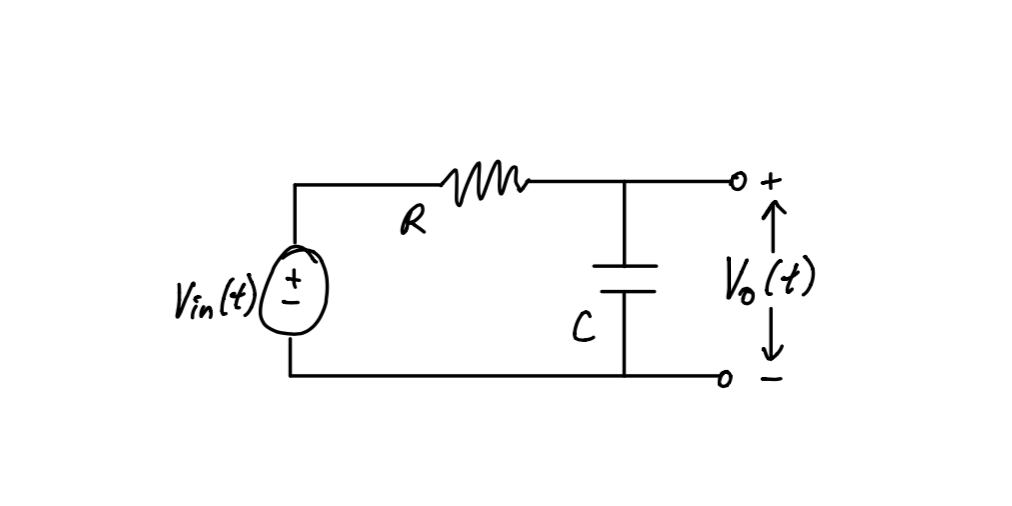
\includegraphics[scale=0.5]{RC.png}
\end{center}

Suppose we have a simple RC circuit as shown above, how can we find the impulse response, (to voltage input $\delta(t)$). Well, we can take advantage of the fact that, for LTI systems, \textbf{the derivative of the unit step response is the impulse response}. This will be proved later in the course.\\
\bigskip
The differential equation governing the behavior of a driven RC circuit is the following: 
\begin{equation}
\dot{V}_0(t)+\frac{V_0(t)}{RC}=\frac{V_{in}(t)}{RC}
\end{equation}

If we set $V_{in}(t) = u(t)$, we can solve the following equation which applies for $t>0$ and apply the initial condition of $V_0(t=0)=0$.
\begin{equation}
\dot{V}_0(t)+\frac{V_0(t)}{RC}=\frac{1}{RC}
\end{equation}
The solution to this differential equation is the following:
\begin{equation}
V_{o}(t)=u(t)(1-e^{-t/RC})
\end{equation}
Now we simply differentiate this unit step response to find the impulse response! It is important to remember that $u(t)$ is a function, with a derivative $\delta(t)$.
\begin{equation}
\hat{D}_tV_{o}(t)=\delta(t)-\delta(t)e^{-t/RC}+\frac{u(t)}{RC}e^{-t/RC}=\frac{u(t)}{RC}e^{-t/RC} = h(t)
\end{equation}
The $\hat{D}_t$ operator represents differentiation with respect to time, and the $u(t)$ is necessary because the solution to both the unit step input and delta function input is only non-zero for $t\geq0$.

\subsection{Convolution \& General LTI System Response}
\subsubsection{Discrete}
Suppose you have a signal $x[n]$ defined by the following array where index $n$ corresponds to $x[n]$:
\begin{verbatim}
[3,33,333,3333,33333,333333]
\end{verbatim}
We could also represent this system in functional notation by the following:
\begin{equation}
x[n]=3\delta[n]+33\delta[n-1]+333\delta[n-2]+3333\delta[n-3]+33333\delta[n-4]+333333\delta[n-5]
\end{equation}
By the same logic, \textbf{any} signal can be represented by a sum of shifted and scaled delta functions. Now, \textbf{if we know the the response of an LTI system to a single delta function, we know the response of the system to any signal!} Since the system is linear and time invariant, all we have to do is scale and shift the impulse response appropriately. The logic is as follows:
\begin{equation}
\delta[n] \rightarrow h[n]
\end{equation}
\begin{equation}
\delta[n-k] \rightarrow h[n-k]
\end{equation}
\begin{equation}
x[k]\delta[n-k] \rightarrow x[k]h[n-k]
\end{equation}
\begin{equation}
x[n]=\sum_{k=-\infty}^{\infty}x[k]\delta[n-k] \rightarrow y[n]=\sum_{k=-\infty}^{\infty}x[k]h[n-k]
\end{equation}
The sum performed in line 28 is defined as the \textit{convolution} of $x[n]$ and $h[n]$ and is commutative. 

\subsubsection{Continuous}
Suppose you have a function $x(t)$ defining an input signal (ex: $u(t)\cos{t}$). By the definition of the $\delta(t)$, we could also represent $x(t)$ by the following expression:
\begin{equation}
x(t)=\int_{-\infty}^{\infty}d\tau\: x(\tau)\delta(t-\tau)
\end{equation}
By the same logic, \textbf{any} continuous signal can be represented by a an integral of shifted and scaled delta functions. Now, \textbf{if we know the the response of an LTI system to a single delta function, we know the response of the system to any signal!} Since the system is linear and time invariant, all we have to do is scale and shift the impulse response appropriately. The logic is as follows:
\begin{equation}
\delta(t) \rightarrow h(t)
\end{equation}
\begin{equation}
\delta(t-\tau) \rightarrow h(t-\tau)
\end{equation}
\begin{equation}
x(\tau)\delta(t-\tau) \rightarrow x(\tau)h(t-\tau)
\end{equation}
\begin{equation}
x(t)=\int_{\infty}^{\infty}d\tau \; x(\tau)\delta(t-\tau) \rightarrow y(t)=\int_{-\infty}^{\infty}d\tau \; x(\tau)h(t-\tau)
\end{equation}
The integral performed in line 33 is defined as the \textit{convolution} of $x(t)$ and $h(t)$ and is commutative. 

\subsubsection{More on Convolution}
Convolution is defined by the following equations for discrete and continuous systems, and denoted by the $*$ operator.
\begin{equation}
x[n]*y[n]=\sum_{k=-\infty}^{\infty}x[k]y[n-k]
\end{equation}
\begin{equation}
x(t)*y(t)=\int_{-\infty}^{\infty}d\tau \; x(\tau)y(t-\tau)
\end{equation}
A graphical representation of convolution can be found \href{https://upload.wikimedia.org/wikipedia/commons/b/b9/Convolution_of_spiky_function_with_box2.gif}{here}.  We will discuss how to find the convolution of simple discrete signals graphically in class.

\section{Frequency Domain}


\subsection{Review of Complex Numbers}
Complex numbers are usually denoted by the following:
\begin{equation}
z = a+jb \qquad \text{where} \quad a, b \in \Re, \quad j \equiv \sqrt{-1}
\end{equation}

We will almost always use Euler's formula to describe and work with complex numbers.
\begin{equation}
\boxed{e^{j \theta} = \cos{\theta}+j\sin{\theta}}
\end{equation}

This equation can be shown to be true by taking the Taylor expansion of $e^{j\theta}$ and comparing it with the well known Taylor expansions of $\cos{\theta}$ and $\sin{\theta}$. 
\begin{equation}
e^{j\theta} = \sum_{n=0}^{\infty} \frac{(j\theta)^n}{n!} = \sum_{m=0}^{\infty} \frac{(j\theta)^{2m}}{(2m)!}+\sum_{k=0}^{\infty} \frac{(j\theta)^{2k+1}}{(2k+1)!}
=\underbrace{ \sum_{m=0}^{\infty} \frac{(-1)^m\theta^{2m}}{(2m)!}}_{\cos{\theta}}+\underbrace{j\sum_{k=0}^{\infty} \frac{(-1)^{k}\theta^{2k+1}}{(2k+1)!}}_{j\sin{\theta}}
\end{equation}

It is easiest to interpret this relationship by visualizing a complex number as a vector in the complex plane. 
\begin{center}
\begin{tikzpicture}[scale=1]
    \begin{scope}[thick,font=\scriptsize]
    % Axes:
    % Are simply drawn using line with the `->` option to make them arrows:
    % The main labels of the axes can be places using `node`s:
    \draw [->] (-5,0) -- (5,0) node [above left]  {$\Re\{z\}$};
    \draw [->] (0,-5) -- (0,5) node [below right] {$\Im\{z\}$};

    % Axes labels:
    % Are drawn using small lines and labeled with `node`s. The placement can be set using options

    \foreach \n in {-4,...,-1,1,2,...,4}{%
        \draw (\n,-3pt) -- (\n,3pt)   node [above] {$\n$};
        \draw (-3pt,\n) -- (3pt,\n)   node [right] {$\n j$};}
    \end{scope}
    % The circle is drawn with `(x,y) circle (radius)`
    % You can draw the outer border and fill the inner area differently.
    % Here I use gray, semitransparent filling to not cover the axes below the circle
    \draw [->] (0,0) -- (2,3);
    \draw [-,dashed, blue] (0,3) -- (2,3);
    \draw [-,dashed, red] (2,0) -- (2,3);
    % Place the equation into the circle:
    \node at (+1,+1.8) {$r$};
    \node [text=blue] at (+1,+3.3) {$a$};
    \node [text=red] at (+2.25,+1.5) {$b$};
    \draw 
    (3,0) coordinate (a) node[right] {}
    -- (0,0) coordinate (b) node[left] {}
    -- (2,3) coordinate (c) node[above right] {}
    pic["$\theta$", draw=orange, ->, angle eccentricity=1.2, angle radius=0.7cm] {angle=a--b--c};
\end{tikzpicture}
\end{center}

We will denote $r, \theta \in \Re$ as the \textit{magnitude} and \textit{phase} of a complex number, respectively. Complex numbers will generally be referred to in the form $re^{j\theta}$. We will also often refer to the \textit{complex conjugate}, which is simply $re^{-j\theta}$, (if the complex number is not in Euler form, \textbf{every} $j$ must be changed to $-j$ to conjugate). You can always find the magnitude squared of a complex number by multiplying the complex number $z$ by its complex conjugate. Interpreting a complex expression geometrically will prove extremely useful when finding $r$ and $\theta$. \\
\bigskip

We will need to know how to use one more tool in this course, the Kronecker delta, $\delta_{ij}$, defined by the following relationship:
\begin{equation}
\delta_{ij} \equiv
\begin{cases} 
      1 & \text{if}\: i=j \\
      0 & \text{else}
   \end{cases}
\end{equation}
  

\subsection{Continuous Fourier Series}
\subsubsection{Real Representation}
Fourier Series are an extremely useful tool in engineering, physics, and mathematics. The theory stems from the idea that any periodic function can be constructed from a sum of weighted harmonics (sines and cosines) of the same periodicity. For example, say you have a square wave with period $T$ on the real number line. Such as the following:
\begin{center}
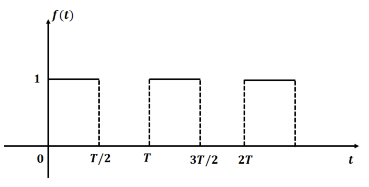
\includegraphics[scale=0.75]{squarewave.png}
\end{center}

Fourier theory proposes that this square wave can be reconstructed from a sum of weighted sines and cosines of the same periodicity, so the following must be true:
\begin{equation}\boxed{
f(t)=\sum_{k=0}^{\infty}a_k\cos{(2\pi kt/T)}+\sum_{k=1}^{\infty}b_k\sin{(2\pi kt/T)}}
\end{equation}
Note that although all of the harmonics don't have $T$ as their minimum period, they are all still periodic with period $T$. Also note that the second sum starts $k$ at index 1 instead of 0 because $sin{(0)}$ is 0.  \\
\smallskip

So how can we find the coefficients $a_k$ and $b_k$? We can take advantage of the orthogonality of all of the harmonics! By orthogonality of the harmonics I mean the following (where $a$ and $b$ are integers:
\begin{equation}
\int_{-T/2}^{T/2}dt\; \cos{(2\pi a t/T)}\cos{(2\pi b t/T)} = \delta_{ab}\frac{T}{2}
\end{equation}
\begin{equation}
\int_{-T/2}^{T/2}dt\; \sin{(2\pi a t/T)}\sin{(2\pi b t/T)} = \delta_{ab}\frac{T}{2}
\end{equation}
\begin{equation}
\int_{-T/2}^{T/2}dt\; \cos{(2\pi a t/T)}\sin{(2\pi b t/T)} = 0
\end{equation}

We can find any $a_n$ by the following method:
\begin{equation}
f(t)=\sum_{k=0}^{\infty}a_k\cos{(2\pi kt/T)}+\sum_{k=1}^{\infty}b_k\sin{(2\pi kt/T)}
\end{equation}
\begin{equation}
f(t)\cos{(2\pi n t/T)}=\sum_{k=0}^{\infty}a_k\cos{(2\pi kt/T)}\cos{(2\pi nt/T)}+\sum_{k=1}^{\infty}b_k\sin{(2\pi kt/T)}\cos{(2\pi n t/T)}
\end{equation}
\begin{equation}
\int_{-T/2}^{T/2}dt\; f(t)\cos{(2\pi n t/T)}=\int_{-T/2}^{T/2}dt\;\big(\sum_{k=0}^{\infty}a_k\cos{(2\pi kt/T)}\cos{(2\pi n t/T)}+\sum_{k=1}^{\infty}b_k\sin{(2\pi kt/T)}\cos{(2\pi n t/T)}\big)
\end{equation}
\begin{equation}
\int_{-T/2}^{T/2}dt\; f(t)\cos{(2\pi n t/T)}=\sum_{k=0}^{\infty}\frac{T}{2}a_k\delta_{kn}
\end{equation}
\begin{equation}
\int_{-T/2}^{T/2}dt\; f(t)\cos{(2\pi n t/T)}=\frac{T}{2}a_n
\end{equation}
\begin{equation}
\boxed{
a_n=\frac{2}{T}\int_{-T/2}^{T/2}dt\; f(t)\cos{(2\pi n t/T)}}
\end{equation}


By the same logic, we can find any $b_m$ by the following method:
\begin{equation}
f(t)=\sum_{k=0}^{\infty}a_k\cos{(2\pi kt/T)}+\sum_{k=1}^{\infty}b_k\sin{(2\pi kt/T)}
\end{equation}
\begin{equation}
f(t)\sin{(2\pi m t/T)}=\sum_{k=0}^{\infty}a_k\cos{(2\pi kt/T)}\sin{(2\pi m t/T)}+\sum_{k=1}^{\infty}b_k\sin{(2\pi kt/T)}\sin{(2\pi m t/T)}
\end{equation}
\begin{equation}
\int_{-T/2}^{T/2}dt\; f(t)\cos{(2\pi m t/T)}=\int_{-T/2}^{T/2}dt\;\big(\sum_{k=0}^{\infty}a_k\cos{(2\pi kt/T)}\sin{(2\pi m t/T)}+\sum_{k=1}^{\infty}b_k\sin{(2\pi kt/T)}\sin{(2\pi m t/T)}\big)
\end{equation}
\begin{equation}
\int_{-T/2}^{T/2}dt\; f(t)\sin{(2\pi n t/T)}=\sum_{k=1}^{\infty}\frac{T}{2}b_k\delta_{kn}
\end{equation}
\begin{equation}
\int_{-T/2}^{T/2}dt\; f(t)\sin{(2\pi m t/T)}=\frac{T}{2}b_n
\end{equation}
\begin{equation}
\boxed{
b_m=\frac{2}{T}\int_{-T/2}^{T/2}dt\; f(t)\sin{(2\pi m t/T)}}
\end{equation}


You can the interact with the reconstruction process of square wave above using the online mathematical tool Desmos \href{https://www.desmos.com/calculator/fpa1cpj0np}{here}. With any finite sum Fourier series, the jump discontinuities of the function will not be perfect, you can read more about this phenomenon \href{https://en.wikipedia.org/wiki/Gibbs_phenomenon}{here}. 

\subsubsection{Complex Representation}
In practice, it is very convenient to represent sines and cosines in complex form instead. Suppose we start with our function reconstruction formula:
\begin{equation}
f(t)=\sum_{k=0}^{\infty}a_k\cos{(2\pi kt/T)}+\sum_{k=1}^{\infty}b_k\sin{(2\pi kt/T)}
\end{equation}
We would like to replace $\cos(x)$ and $\sin(x)$ with their complex representations:
\begin{equation}
\cos{x}=\frac{e^{jx}+e^{-jx}}{2} \: \: \: \: \& \: \: \: \: \sin{x}=\frac{e^{jx}-e^{-jx}}{2j} 
\end{equation}
If we plug these relationships into our reconstruction formula we get: 
\begin{equation}
f(t)=\sum_{k=0}^{\infty}a_k\big(\frac{e^{j2\pi kt/T}+e^{-j2\pi kt/T}}{2} \big)+\sum_{k=1}^{\infty}b_k\big(\frac{e^{j2\pi kt/T}-e^{-j2\pi kt/T}}{2j} \big)
\end{equation}
Grouping terms:
\begin{equation}
f(t)=\sum_{k=0}^{\infty}\frac{a_k-jb_k}{2}e^{j2\pi kt/T}+\frac{a_k+jb_k}{2}e^{-j2\pi kt/T}
\end{equation}
Where we are allowed to group the sums because the second sum starting at 0 is inconsequential. This function can be re-written as:
\begin{equation}
f(t)=\sum_{k=0}^{\infty}\frac{a_k-jb_k}{2}e^{j2\pi kt/T}+\sum_{k=0}^{-\infty}\frac{a_{-k}+jb_{-k}}{2}e^{j2\pi kt/T}
\end{equation}
And even further simplified as:
\begin{equation}
\boxed{
f(t)=\sum_{n=-\infty}^{\infty}c_n e^{j2\pi nt/T}
}
\end{equation}
Where
\begin{equation}
c_n =
\begin{cases} 
      (a_n-jb_n)/2 & n>0 \\
      (a_{-n}+jb_{-n})/2 & n<0\\
      a_0 & n=0
   \end{cases}
\end{equation}
Fortunately, there is still a very simple way to calculate the $c_n$ coefficients without using $a_n$ and $b_n$. We must take advantage of the following fact:
\begin{equation}
\int_{-T/2}^{T/2}dt \; e^{j2\pi mt/T} = T\delta_{0,m} \: \: m \in \mathbb{Z}
\end{equation}
This can be shown to be true by expanding the complex exponential into cosine and sine. Therefore, by the same logic as we used in the real representation of Fourier Series, we can find any $c_m$:
\begin{equation}
f(t)=\sum_{n=-\infty}^{\infty}c_n e^{j2\pi nt/T}
\end{equation}
\begin{equation}
f(t)e^{-j2\pi mt/T}=\sum_{n=-\infty}^{\infty}c_n e^{j2\pi nt/T}e^{-j2\pi mt/T}
\end{equation}
\begin{equation}
\int_{-T/2}^{T/2}dt\; f(t)e^{-j2\pi mt/T}=\int_{-T/2}^{T/2}dt\; \big(\sum_{n=-\infty}^{\infty}c_n e^{j2\pi nt/T}e^{-j2\pi mt/T}\big)
\end{equation}
\begin{equation}
\int_{-T/2}^{T/2}dt\; f(t)e^{-j2\pi mt/T}=\int_{-T/2}^{T/2}dt\; \sum_{n=-\infty}^{\infty}c_n e^{j2\pi (n-m)t/T}
\end{equation}
\begin{equation}
\int_{-T/2}^{T/2}dt\; f(t)e^{-j2\pi mt/T}=\sum_{n=-\infty}^{\infty}Tc_n\delta_{nm}
\end{equation}
\begin{equation}
\int_{-T/2}^{T/2}dt\; f(t)e^{-j2\pi mt/T}=Tc_m
\end{equation}
\begin{equation}
\boxed{
c_m=\frac{1}{T}\int_{-T/2}^{T/2}dt\; f(t)e^{-j2\pi mt/T}}
\end{equation}

From now on, we will only use Fourier theory in the complex domain.

\subsection{Discrete Fourier Transform}
The discrete Fourier transform is the discrete analog of the continuous Fourier series. The theory stems from the fact that the vectors:
\begin{equation}
u_k = \Big[ e^{j2\pi kn/N}|n \in \{ 0,1,...,N-1\} \Big]^T
\end{equation}
form an orthogonal basis over the set of N-dimensional complex vectors, (this is basically saying that sines and cosines of the same frequency $k$ form a basis, but again, complex exponentials are much easier to work with). This fact will not be proven in this course. Note that $u_k = u_{k+N}$; this  is a key cyclic property of this basis.\\

If the vectors $u_k$ form a basis for an $n$ dimensional complex space, we should be able to construct any $n$ dimensional vector from their linear superposition. Suppose we have an $N$ dimensional vector $x[n]$ that is the input to one of our LTI systems discussed in section 1. We should be able to construct it as the following:
\begin{equation}
\boxed{
x[n]=\frac{1}{N}\sum_{k=0}^{N-1}\hat{X}[k]e^{j2\pi kn/N}}
\end{equation}
Where $\hat{X}[k]$ denotes the coefficients of our basis vectors, also known as the \textbf{Discrete Fourier Transform} of $x[n]$. The division by $N$ is simply a scale necessary scale factor due to the nature of the construction of $\hat{X}[k]$. Note again that, given this definition, $x[n]=x[n+N]$; the discrete Fourier transform (DFT) assumes periodicity similar to the continuous Fourier series. \\

So how can we find $\hat{X}[k]$? We again take advantage of the orthogonality of our chosen basis vectors. 
\begin{equation}
u_k^Tu_{k'} = \sum_{n=0}^{N-1}e^{j2\pi kn/N}e^{-j2\pi k' n/N}=\sum_{n=0}^{N-1}e^{j2\pi (k-k')n/N}=N\delta_{k,k'}
\end{equation}
This can be calculated explicitly, but it is sufficient to remember that $e^{j\theta}=\cos{\theta}+j\sin{\theta}$ and think about summing $N$ evenly spaced points along one period of a sine wave; there is the same amount of positive function as there is negative! Given this information, we may now find any $\hat{X}[k']$ as follows:
\begin{equation}
x[n]=\frac{1}{N}\sum_{k=0}^{N-1}\hat{X}[k]e^{j2\pi kn/N}
\end{equation}
\begin{equation}
x[n]e^{-j2\pi k' n/N}=\frac{1}{N}\sum_{k=0}^{N-1}\hat{X}[k]e^{j2\pi kn/N}e^{-j2\pi k' n/N}
\end{equation}
\begin{equation}
\sum_{n=0}^{N-1}x[n]e^{-j2\pi k' n/N}=\frac{1}{N}\sum_{n=0}^{N-1}\sum_{k=0}^{N-1}\hat{X}[k]e^{j2\pi (k-k')n/N}
\end{equation}
\begin{equation}
\sum_{n=0}^{N-1}x[n]e^{-j2\pi k' n/N}=\frac{1}{N}\sum_{k=0}^{N-1}\hat{X}[k]N\delta_{k,k'}
\end{equation}
\begin{equation}
\boxed{
\hat{X}[k']=\sum_{n=0}^{N-1}x[n]e^{-j2\pi k' n/N}}
\end{equation}

This is the inner product of our vector $x[n]$ with one of our orthogonal basis vectors! \textbf{It is important to remember that $n$ and $k$ are sample number and sample frequency respectively, and when working with actual data it is useful to convert to actual temporal/spatial values and frequencies}.

\subsection{Continuous Fourier Transform}
We are now going to discuss what is known as the Continuous Fourier Transform, commonly just Fourier Transform. This can be thought of as the limit of the Continuous Fourier Series as the period $T$ is extended to $\infty$. The FT is useful because it allows to analyze the frequency content of non-periodic functions! If we start with the Continuous Fourier Series expressions:
\begin{equation}
c_m=\frac{1}{T}\int_{-T/2}^{T/2}dt\; f(t)e^{-j2\pi mt/T}\: \: \: \& \:  \: \: f(t)=\sum_{n=-\infty}^{\infty}c_n e^{j2\pi nt/T}
\end{equation}
We can move the $\frac{1}{T}$ to the temporal construction equation as follows:
\begin{equation}
c_m=\int_{-T/2}^{T/2}dt\; f(t)e^{-j2\pi mt/T}\:  \: \: \& \: \: \: f(t)=\sum_{n=-\infty}^{\infty}\frac{c_n}{T} e^{j2\pi nt/T}
\end{equation}
Then, taking the limit as $T \rightarrow \infty$ of the left equation:
\begin{equation}
\hat{f}(\xi)=\int_{-\infty}^{\infty}dt\; f(t)e^{-j2\pi \xi t}
\end{equation}
Where we have defined $\xi$ to be the (now continuous) frequency $\frac{m}{T}$. The temporal function reconstruction then becomes:
\begin{equation}
f(t)=\sum_{n=-\infty}^{\infty}\frac{1}{T}\hat{f}(\frac{n}{T}) e^{j2\pi nt/T}
\end{equation}
When taking the limit of $T\rightarrow \infty$ this sum is interpreted as the Riemann sum of the argument with step size $\frac{1}{T}$
\begin{equation}
f(t)=\lim_{T\rightarrow \infty}\sum_{n=-\infty}^{\infty}\frac{1}{T}\hat{f}(\frac{n}{T}) e^{j2\pi nt/T} = \int_{-\infty}^{\infty} d\xi \; \hat{f}(\xi) e^{j2\pi \xi t}
\end{equation}
It is common to use the Fourier Transform in terms of angular frequency $\omega=2\pi \xi$, so we can do a quick change of variables to get the preferred form.
\begin{equation}\boxed{
\hat{f}(\omega)=\int_{-\infty}^{\infty}dt\; f(t)e^{-j\omega t}}
\end{equation}
\begin{equation}\boxed{
f(t)=\frac{1}{2\pi}\int_{-\infty}^{\infty} d\omega \; \hat{f}(\omega) e^{j\omega t}}
\end{equation}

The Fourier Transform $\hat{f}(\omega)$ of a function carries with it all of the information needed to describe that function. We are simply changing our basis from spatial/temporal to harmonic. The formula for constructing $\hat{f}(\omega)$ should also make sense intuitively because continuous complex exponentials form a basis for the infinite dimensional real number line! Therefore, we should be able to \textit{pick out} the coefficients of this basis by taking the inner product with each of the basis vectors! 

\subsection{Discrete Time Fourier Transform}
The Discrete Time Fourier Transform is considered the extension of DFT as $N\rightarrow \infty$. The $\frac{k}{N}$ becomes a continuous variable $\xi$, similar to how the Fourier Series was extended to the Fourier Transform. The DTFT is calculated as follows:
\begin{equation}
\lim_{N\rightarrow \infty}\hat{X}[k]=\lim_{N\rightarrow \infty}\sum_{n=0}^{N-1}x[n]e^{-j2\pi k n/N}
\end{equation}
The following sum will extend from $-\infty$ to $\infty$ because the sum from $0$ to $N$ is actually a sum over any single period of our input signal. 
\begin{equation}
\hat{X}(\xi)=\sum_{n=-\infty}^{\infty}x[n]e^{-j2\pi \xi n}
\end{equation}
We again prefer to use angular frequency and define the new variable $\Omega=2\pi \xi$. 
\begin{equation}\boxed{
\hat{X}(\Omega)=\sum_{n=-\infty}^{\infty}x[n]e^{-j\Omega n}}
\end{equation}
If $N\rightarrow \infty$, how should we calculate $x[n]$ from our DTFT? We will make the same extension to a Riemann sum as we did for the Fourier Transform. 
\begin{equation}
x[n]=\frac{1}{N}\sum_{k=0}^{N-1}\hat{X}[k]e^{j2\pi kn/N}
\end{equation}
\begin{equation}
x[n]=\lim_{N\rightarrow \infty}\frac{1}{N}\sum_{k=0}^{N-1}\hat{X}[k]e^{j2\pi kn/N}
\end{equation}
\begin{equation}
x[n]=\int_{0}^{1}d\xi \hat{X}(\xi)e^{j2\pi \xi n}
\end{equation}
And finally switch to $\Omega=2\pi \xi$.
\begin{equation}\boxed{
x[n]=\frac{1}{2\pi}\int_{0}^{2\pi}d\Omega\; \hat{X}(\Omega)e^{j\Omega n}}
\end{equation}

It is important to note that the DFT can be considered uniform samples of the DTFT, and that zero-padding a signal before taking the DFT brings it closer to the DTFT. A visual representation of this can be found \href{https://upload.wikimedia.org/wikipedia/commons/c/ca/Fourier_transform\%2C_Fourier_series\%2C_DTFT\%2C_DFT.gif}{here}

\section{Relationship between Convolution \& Multiplication}
One very important part of signal analysis is the fact that multiplication in the frequency domain corresponds to convolution in the spatial/temporal domain, and vice versa.  This is an extremely important tool when it comes to finding the output and impulse response of LTI systems. 

\subsection{Aperiodic Continuous Functions}
We can show that multiplication in the frequency domain is equal to convolution of continuous functions in the time/spatial domain as follows:\\

Suppose we multiply the Fourier transforms of two functions $f(t)$ and $g(t)$, what is the resulting temporal function?
\begin{equation}
\frac{1}{2\pi}\int_{-\infty}^{\infty}d\omega \; \hat{f}(\omega)\hat{g}(\omega)e^{j\omega t}=\frac{1}{2\pi}\int_{-\infty}^{\infty}d\omega \; \int_{-\infty}^{\infty}dt_1\; f(t_1)e^{-j\omega t_1}\int_{-\infty}^{\infty}dt_2\; g(t_2)e^{-j\omega t_2}e^{j\omega t}
\end{equation}
\begin{equation}
= \int_{-\infty}^{\infty}dt_1\; f(t_1)\int_{-\infty}^{\infty}dt_2\; g(t_2)\frac{1}{2\pi}\int_{-\infty}^{\infty}d\omega \;e^{j\omega (t-t_1-t_2)}
\end{equation}
The next step uses the Fourier transform of $\delta(t-t_0)$. 
\begin{equation}
= \int_{-\infty}^{\infty}dt_1\; f(t_1)\int_{-\infty}^{\infty}dt_2\; g(t_2)\delta(t-t_1-t_2)
\end{equation}
\begin{equation}
= \int_{-\infty}^{\infty}dt_1\; f(t_1)g(t-t_1)
\end{equation}
Therefore,
\begin{equation}
\boxed{
\hat{f}(\omega)\hat{g}(\omega)\Longleftrightarrow f(t)*g(t)
}
\end{equation}

The inverse relationship can also be shown (multiplication in the temporal domain corresponds to convolution in the frequency domain). \\


Why do we care? We can do many useful things with this tool, such as find the output of a continuous LTI system by multiplying the FT of the input and unit impulse response! We can also filter an incoming signal (attenuate the power of certain frequencies) by having a very specific impulse response! More on filtering later. 

\subsection{Aperiodic Discrete Functions}
We can show that multiplication in the frequency domain is equal to convolution of discrete functions in the time/spatial domain as follows:\\

Suppose we multiply the DTFTs of two signals $f[n]$ and $g[n]$, what is the resulting signal?
\begin{equation}
\frac{1}{2\pi}\int_{0}^{2\pi}d\Omega \; \hat{F}(\Omega)\hat{G}(\Omega)e^{j\Omega n}=\frac{1}{2\pi}\int_{0}^{2\pi}d\Omega \; \sum_{n_1=-\infty}^{\infty} f[n_1]e^{-j\Omega n_1}\sum_{n_2=-\infty}^{\infty}g[n_2]e^{-j\Omega n_2}e^{j\Omega n}
\end{equation}
\begin{equation}
=\sum_{n_1=-\infty}^{\infty} f[n_1]\sum_{n_2-\infty}^{\infty}g[n_2]\frac{1}{2\pi}\int_{0}^{2\pi}d\Omega \; e^{j\Omega (n-n_1-n_2)}
\end{equation}
The next step uses the DFT of $\delta[n-n_0]$. 
\begin{equation}
=\sum_{n_1=-\infty}^{\infty} f[n_1]\sum_{n_2-\infty}^{\infty}g[n_2]\delta[n-n_1-n_2]
\end{equation}
\begin{equation}
=\sum_{n_1=-\infty}^{\infty} f[n_1]\sum_{n_2-\infty}^{\infty}g[n-n_1]
\end{equation}
Therefore,
\begin{equation}\boxed{
\hat{F}(\Omega)\hat{G}(\Omega) \Longleftrightarrow f[n]*g[n]}
\end{equation}

Again, the inverse relationship is also true. \\

We can use this tool easily manipulate and solve our LTI systems!

\subsection{Periodic Continuous Functions}
This useful property is a little different when dealing with Periodic functions, as we will see below with the Fourier Series. What if we multiply each value of the Fourier Series of two (periodic in T) signals $f(t)$ and $g(t)$, with Fourier Series coefficients $a_n$ and $b_n$ respectively. We will call the resulting temporal function $s(t)$. 
\begin{equation}
s(t)=\sum_{n=-\infty}^{\infty}a_n b_n e^{j2\pi nt/T} 
\end{equation}
\begin{equation}
s(t)= \sum_{n=-\infty}^{\infty}\frac{1}{T}\int_{-T/2}^{T/2}dt_1\; f(t_1)e^{-j2\pi mt_1/T}\frac{1}{T}\int_{-T/2}^{T/2}dt_2\; g(t_2)e^{-j2\pi mt_2/T}e^{j2\pi nt/T} 
\end{equation}
\begin{equation}
s(t)= \frac{1}{T}\int_{-T/2}^{T/2}dt_1\; f(t_1)\int_{-T/2}^{T/2}dt_2\; g(t_2)\frac{1}{T}\sum_{n=-\infty}^{\infty}e^{j2\pi n(t-t_1-t_1)/T} 
\end{equation}
The next step uses the Fourier Series of a periodic $\delta(t-t_0)$. 
\begin{equation}
s(t)= \frac{1}{T}\int_{-T/2}^{T/2}dt_1\; f(t_1)\int_{-T/2}^{T/2}dt_2\; g(t_2)\sum_{k=-\infty}^{\infty}\delta(t-t_1-t_2-kT)
\end{equation}
\begin{equation}
s(t)= \frac{1}{T}\int_{-T/2}^{T/2}dt_1\; f(t_1)\sum_{k=-\infty}^{\infty}g(t-t_1-kT)
\end{equation}
Note that
\begin{equation}
\sum_{k=-\infty}^{\infty}g(t-t_1-kT)
\end{equation}
is just periodic and shifted $g(t)$! Therefore, we can rewrite the eq. 107 as:
\begin{equation}
s(t)= \frac{1}{T}\int_{-T/2}^{T/2}dt_1\; f(t_1)g\big((t-t_1)\; \text{mod}\; T\big)
\end{equation}
\begin{equation}
\boxed{
a_nb_n\Longleftrightarrow \frac{1}{T}f(t)\circledast g(t)}
\end{equation}
This operation is defined as periodic or \textbf{circular convolution}, and is denoted by the $\circledast$ operator. The inverse relationship is also true in this case as well, (multiplication in time corresponds to circular convolution in frequency). 

\subsection{Periodic Discrete Functions}
The same property applies to Discrete Periodic Functions, or functions that are assumed to be period by taking the Discrete Fourier Transform. If we multiply each value of the DFT of two signals $f[n]$ and $g[n]$, and then take the inverse DFT, we will again be left with the circular convolution of the two signals. If we denote the resulting signal as $s[n]$, this can be proved similarly to how we proved the circular convolution property of the Fourier Series. 
\begin{equation}
s[n]=\frac{1}{N}\sum_{k=0}^{N-1}\hat{F}[k]\hat{G}[k]e^{j2\pi kn/N}
\end{equation}
\begin{equation}
s[n]=\frac{1}{N}\sum_{k=0}^{N-1}\sum_{n_1=0}^{N-1}f[n_1]e^{-j2\pi k n_1/N}\sum_{n_2=0}^{N-1}g[n_2]e^{-j2\pi k n_2/N}e^{j2\pi kn/N}
\end{equation}
\begin{equation}
s[n]=\sum_{n_1=0}^{N-1}f[n_1]\sum_{n_2=0}^{N-1}g[n_2]\frac{1}{N}\sum_{k=0}^{N-1}e^{j2\pi k(n-n_1-n_2)/N}
\end{equation}
The next step uses the Discrete Fourier Transform of a periodic $\delta[t-t_0]$. 
\begin{equation}
s[n]=\sum_{n_1=0}^{N-1}f[n_1]\sum_{n_2=0}^{N-1}g[n_2]\sum_{k=-\infty}^{\infty}\delta[n-n_1-n_2-kN]
\end{equation}
\begin{equation}
s[n]=\sum_{n_1=0}^{N-1}f[n_1]\sum_{k=-\infty}^{\infty}g[n-n_1-kN]
\end{equation}
Note that 
\begin{equation}
\sum_{k=-\infty}^{\infty}g[n-n_1-kN]
\end{equation}
is just periodic and shifted $g[n]$! Therefore, we can rewrite the eq. 115 as:
\begin{equation}
s[n]=\sum_{n_1=0}^{N-1}f[n_1]g[(n-n_1)\mod N]
\end{equation}
\begin{equation}
\boxed{
\hat{F}[k]\hat{G}[k]\Longleftrightarrow f[n]\circledast g[n]}
\end{equation}

The inverse relationship is also true in this case as well, (multiplication in time corresponds to circular convolution in frequency). 

\subsection{Application to LTI Systems}
We now have a new and extremely powerful tool. Suppose we know the impulse response of a particular LTI system, and we know the input to the system. We have already learned that we can calculate the output that system by convolving our input with our impulse response (section 1.4). Alternatively, we can now take the Fourier Transform of our input and impulse response, an $\mathcal{O}(n\log(n))$ operation for the DFT, multiply them, and simply take the inverse Fourier Transform to find out the output! \\

\subsubsection{Discrete}

For example, suppose we have an input to a discrete system $x[n]$, and impulse response $h[n]$ as shown below:
\begin{center}
\begin{tikzpicture}[auto, node distance=2cm,>=latex']
    \node [input, name=input](input) {$x[n]$};
    \node [block, right of=input] (sum) {LTI System};
    \node [output, name=output, right of=sum](output) {$y[n]$};
    \draw [blue,->, text=black](input) -- node{$x[n]$}(sum);
    \draw [blue,->,text=black] (sum) -- node {$y[n]$} (output);
\end{tikzpicture}
\end{center}

We can easily calculate y[n] by performing the following steps. First, find the DTFT of the input $x[n]$ and the unit impulse response $h[n]$:
\begin{equation}
\hat{X}(\Omega)=\sum_{n=-\infty}^{\infty}x[n]e^{-j\Omega n} \: \: \: \: \& \: \: \: \: \hat{H}(\Omega)=\sum_{n=-\infty}^{\infty}h[n]e^{-j\Omega n}
\end{equation}
Then simply take the inverse DTFT of their product to find y[n]!
\begin{equation}
y[n] = \frac{1}{2\pi}\int_{0}^{2\pi}d\Omega \; \hat{X}(\Omega)\hat{H}(\Omega)e^{j\Omega n}
\end{equation}
You can also simply describe $y[n]$ by its frequency space representation $\hat{Y}(\Omega)$. 
\begin{equation}
\hat{Y}(\Omega)= \hat{H}(\Omega)\hat{X}(\Omega)
\end{equation}
This is starting to look very similar to the operator notation described in chapter 1!\\

Example:
\smallskip

Suppose you are a given a signal that represents an audio recording in from an area that has a very pronounced echo. You are also given the original audio signal without the echo. The relationship between the input audio signal and the output audio signal can be modeled as an LTI system! Therefore, if you solve for the unit impulse response of the system, you can theoretically remove the echo from any recorded signal!

\subsubsection{Continuous}
The same methodology applies to continuous LTI systems as well. For example, suppose we have an input to a continuous system $x(t)$, and impulse response $h(t)$ as shown below:
\begin{center}
\begin{tikzpicture}[auto, node distance=2cm,>=latex']
    \node [input, name=input](input) {$x(t)$};
    \node [block, right of=input] (sum) {LTI System};
    \node [output, name=output, right of=sum](output) {$y(t)$};
    \draw [blue,->, text=black](input) -- node{$x(t)$}(sum);
    \draw [blue,->,text=black] (sum) -- node {$y(t)$} (output);
\end{tikzpicture}
\end{center}

We can easily calculate y(t) by performing the following steps. First, find the Fourier Transform  of the input $x(t)$ and the unit impulse response $h(t)$:
\begin{equation}
\hat{x}(\omega)=\int_{-\infty}^{\infty}dt\; x(t)e^{-j\omega t} \: \: \: \: \& \: \: \: \: \hat{h}(\omega)=\int_{-\infty}^{\infty}dt\; ht(t)e^{-j\omega t}
\end{equation}
Then simply take the inverse Fourier Transform of their product to find y(t)!
\begin{equation}
y(t) = \frac{1}{2\pi}\int_{-\infty}^{\infty}d\omega \; \hat{x}(\omega)\hat{h}(\omega)e^{j\omega t}
\end{equation}
You can also simply describe $y(t)$ by its frequency space representation $\hat{y}(\omega)$. 
\begin{equation}
\hat{y}(\omega)= \hat{h}(\omega)\hat{x}(\omega)
\end{equation}

Many applications of this will be described when we discuss filtering.

\subsection{More on Circular Convolution}
The same LTI system application applies to the Discrete Fourier Transform \& Fourier Series, unfortunately things are much more complicated due to the nature of circular convolution and the fact that out signals need to be the same length (each Fourier coefficient needs to be multiplied by another). \\

One way to apply the LTI system methodology is by zero padding your signals so that they are not only the same length, but twice as long as the longest signal! This is because the number of non-zero values in the convolution of two signals of length $N$ is $2N-1$. The problem with circular convolution is shown graphically below.\\

Suppose we want to calculate the circular convolution of two signals of the same length $x[n]$ and $y[n]$: 
\begin{verbatim}
x[n] = [a, b, c, d]
\end{verbatim}

\begin{verbatim}
y[n] = [e, f, g, h]
\end{verbatim}

One more intuitive way to think about this is by the following diagram:
\begin{center}
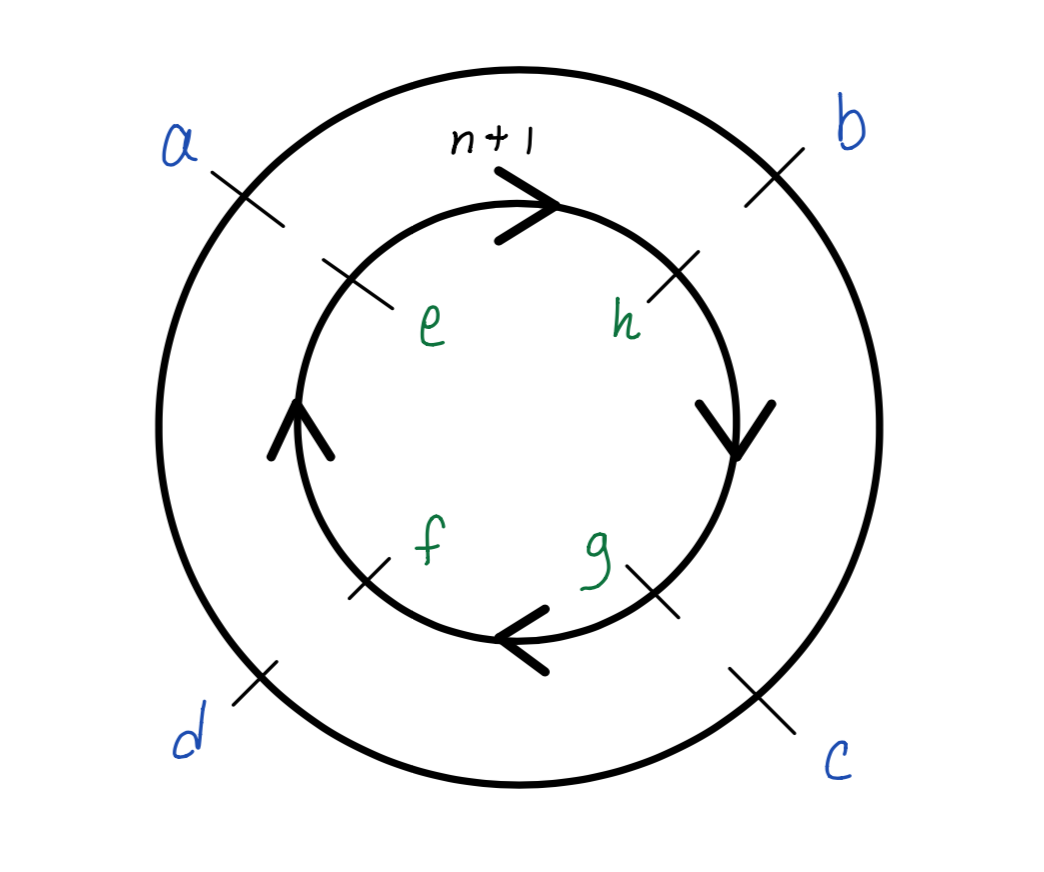
\includegraphics[scale=0.485]{circ.png}
\end{center}
The signals $x[n]$ \& $y[n]$ are represented in blue and green respectively. We can calculate the circular convolution of the two signals by multiplying all of the values that are adjacent along the two circles! We can advance to the next result of the convolution by rotating the inner circle clockwise as shown by the arrows. This diagram should clearly show you that there will be unwanted overlap during the convolution calculation. 

As you can see, the result of such a convolution is most definitely different from the convolution of an input with an impulse response to find the output. If we simply zero pad each signal to twice their original length, we will end up with the proper (non-circular) convolution.
\begin{verbatim}
x[n] = [a, b, c, d, 0, 0, 0, 0]
\end{verbatim}

\begin{verbatim}
y[n] = [e, f, g, h, 0, 0, 0, 0]
\end{verbatim}
Resulting in the new diagram: 
\begin{center}
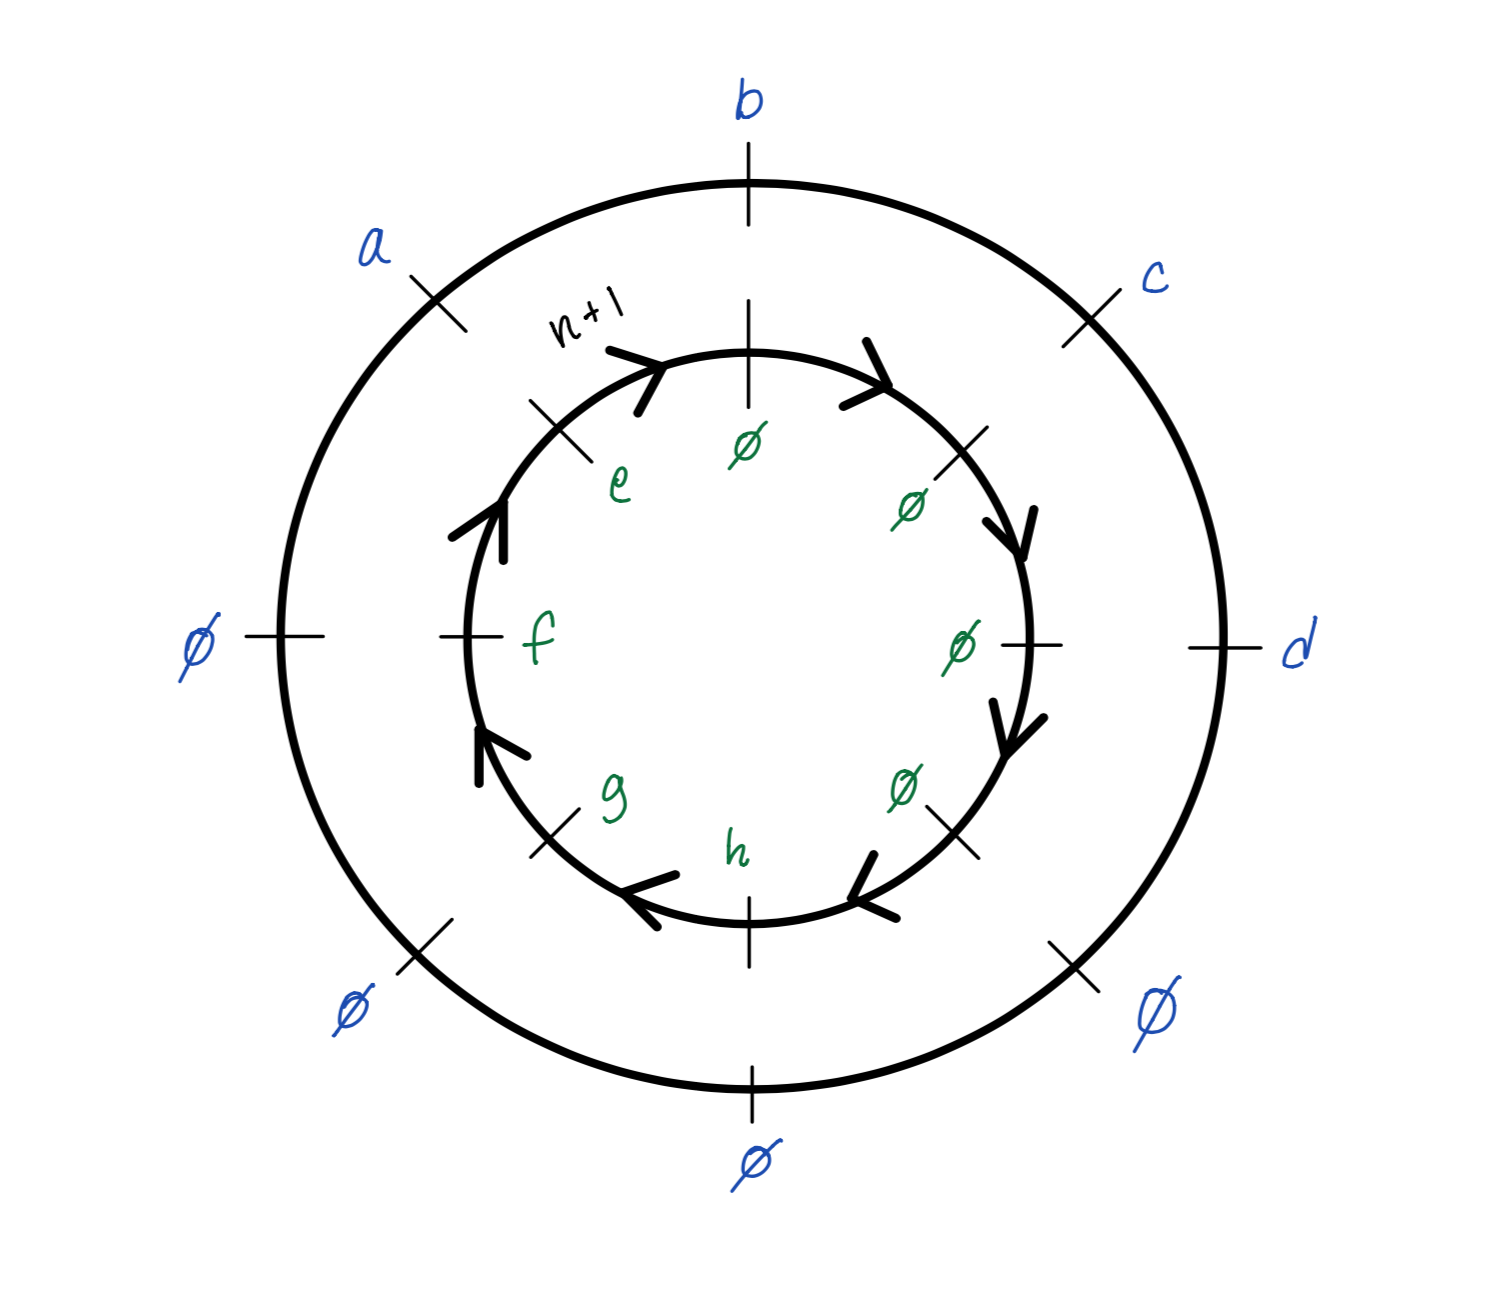
\includegraphics[scale=0.39]{circfixed.png}
\end{center}

Now that the two signals have been zero-padded to twice their length, as the inner circle rotates around to $N=8$ different positions, there will be no unwanted overlap, and the result of our circular convolution will be the same as the result of the output of an LTI system!


\section{Simple Filtering \& Bode Plots}
An extremely useful application of the fact that convolution in time domain corresponds to multiplication in the frequency domain is the ability to remove certain frequency components from LTI inputs! We will call this process \textbf{filtering}.\\

Example:\\
Suppose we are making a high power audio system and we want to send the low frequency components to a different speaker than the high frequency components? Without the use of filtering we might need separate signals representing each part of the music, each recorded separately. \\

So how do we go about filtering signals?

\subsection{Discrete Time}
In order to accomplish filtering with discrete signals it makes most sense to use the Discrete Time Fourier Transform as opposed to the Discrete Fourier Transform. The DFT requires many conditions to be met in order for us to apply a filter; we must know the length of the input and the unit impulse response of our filter must be the same, we have to deal with the unfortunate effects of circular convolution, etc. We will only go into detail regarding simple filters designed using the DTFT. \\

Suppose we want to remove all of the frequency components with a magnitude greater than $\Omega_C$ of a discrete input signal. This operation corresponds to multiplying the DTFT of our input, $\hat{X}(\Omega)$, with the following DTFT:

\begin{equation}
\hat{H}(\Omega) \equiv
\begin{cases} 
      1 & |\Omega| < \Omega_C \\
      0 & otherwise
\end{cases}
\end{equation}

\begin{center}
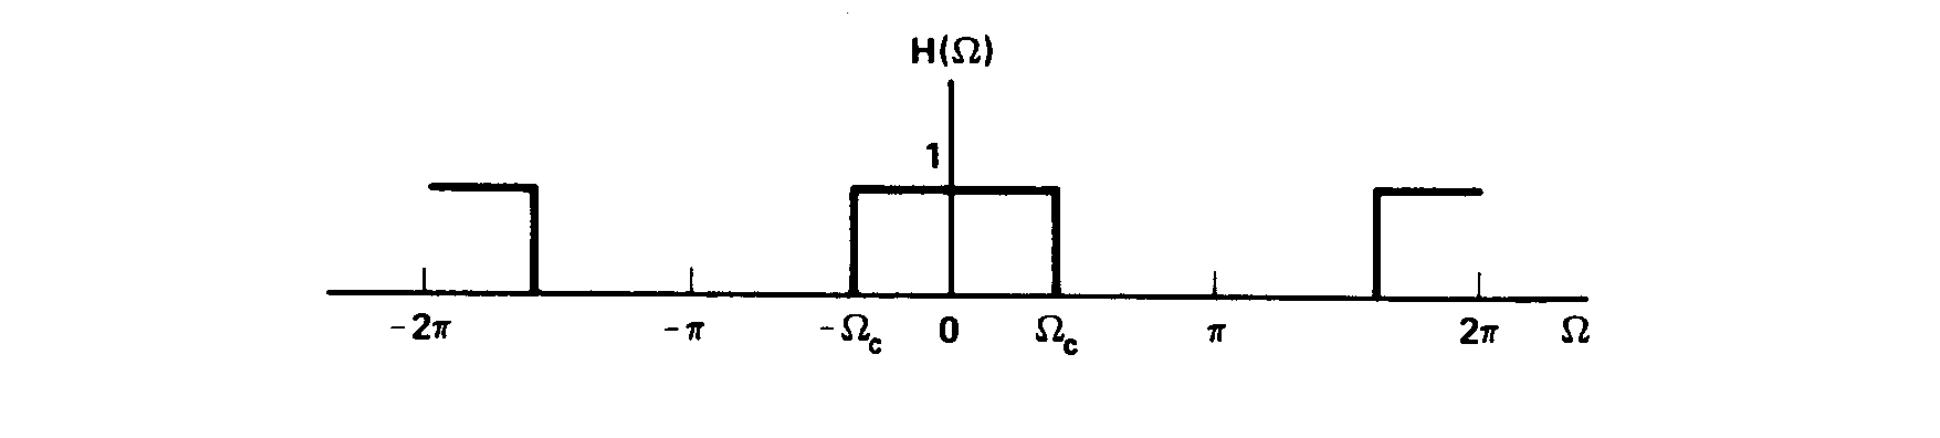
\includegraphics[scale=0.39]{lowpass_ideal_omega.png}
\end{center}

We refer to this as a \textbf{lowpass filter}. The region with value 1 is referred to as the \textbf{bandpass region}, and the region with value zero is referred to as the \textbf{bandstop region}. In fact, this particular filter is an \textit{ideal lowpass filter}, since it perfectly performs the lowpass operation with infinite cutoff slope and completely flat bandpass and bandstop regions.\\
\smallskip

If we want to perform this filtering operation on our incoming discrete signal $x[n]$, we can start with our convolution/multiplication relationship. 
\begin{equation}
x[n]*h[n] \Longleftrightarrow \hat{X}(\Omega)\hat{H}(\Omega)
\end{equation}
Therefore, we must find the impulse response of our ideal lowpass filter by taking the Inverse DFT of $\hat{H}(\Omega)$:
\begin{equation}
h[n]=\frac{1}{2\pi}\int_{-\Omega_C}^{\Omega_C}d\Omega \; e^{j\Omega n}
\end{equation}
\begin{equation}
h[n]=\frac{1}{j2\pi n }\big[ e^{j\Omega n}\big]_{-\Omega_C}^{\Omega_C}
\end{equation}
\begin{equation}
h[n]=\frac{1}{j2\pi n }\big[ e^{j\Omega_C n}-e^{-j\Omega_C n}\big]
\end{equation}
\begin{equation}
h[n]=\frac{2j\sin{(\Omega_C n)}}{j2\pi n }
\end{equation}
\begin{equation}
h[n]=\frac{\sin{(\Omega_C n)}}{\pi n }
\end{equation}

The impulse response $h[n]$ of our filter is known as a \textit{sinc function} and is represented graphically below:
\begin{center}
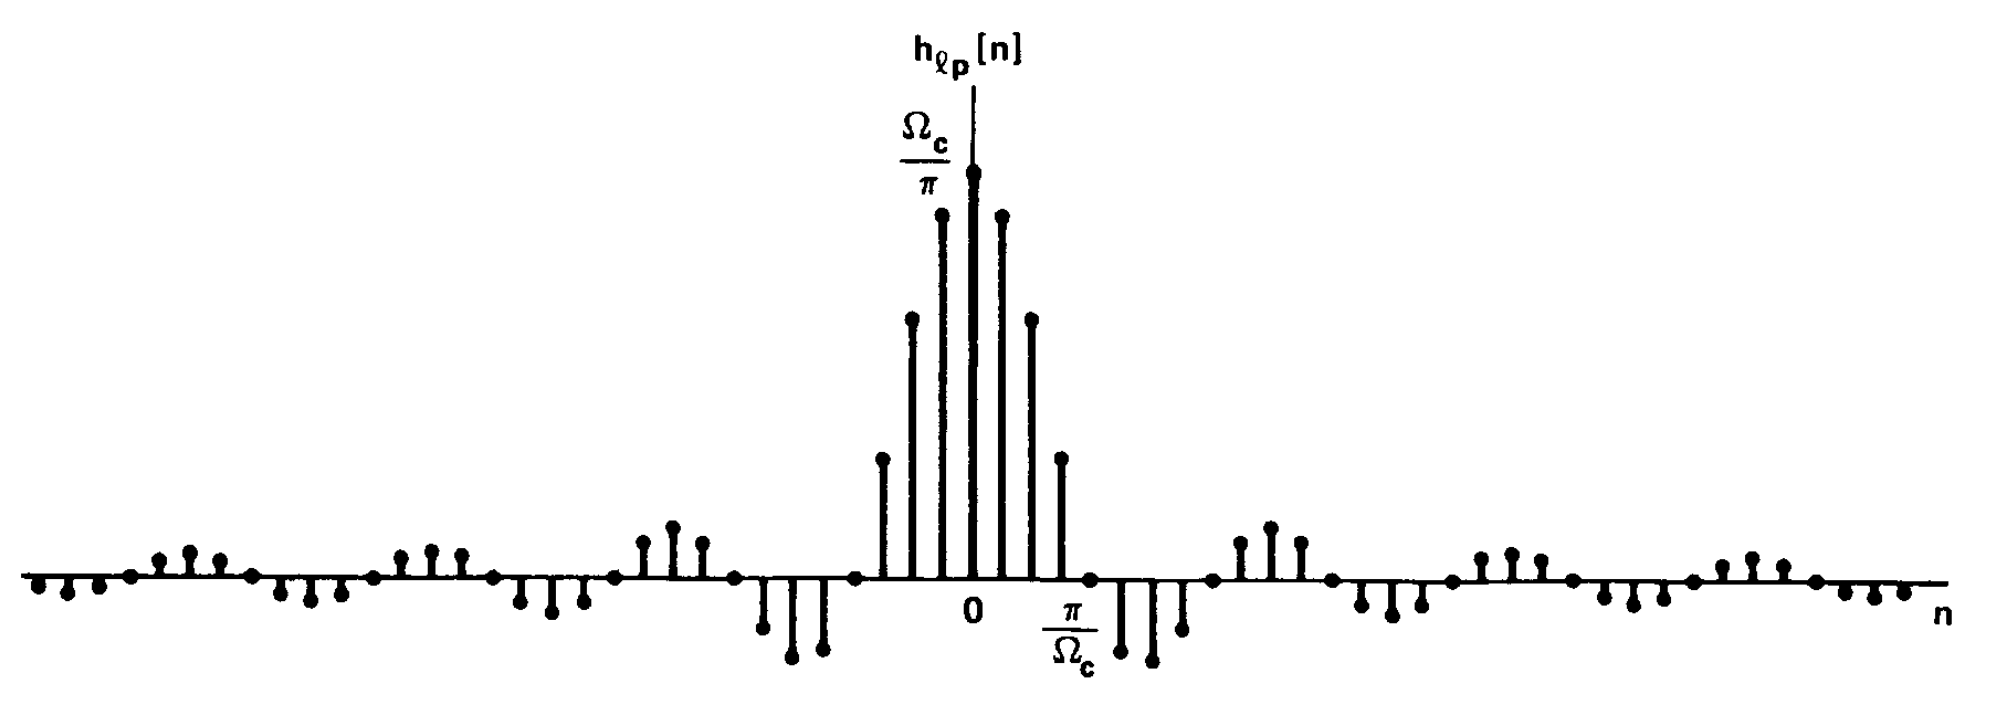
\includegraphics[scale=0.39]{lowpass_ideal_n.png}
\end{center}
Now, when this impulse response is convolved with any input signal $x[n]$, it will completely remove all frequency components with a magnitude greater than $\Omega_C$.\\

*It is important to note that this impulse response is non-causal, meaning the output at time $n$ depends on inputs at times ahead of $n$. In fact, an ideal lowpass filter depends on inputs at times infinitely ahead of $n$. This can not be good, and is one of the reasons why an ideal lowpass filter is not used in practice. Another reasons why the ideal lowpass filter would not be used is because its  impulse response is infinite in the other direction; the convolution would take forever to implement. \\

We will not go into further depth regarding discrete filtering as the design of advanced filters is a very difficult and complex topic. \\

You will calculate the impulse response of an ideal highpass filter in a homework assignment.

\subsection{Continuous Time}
Filters are also a very important concept in continuous time systems. We again start with our convolution/multiplication relationship.
\begin{equation}
f(t)*g(t) \Longleftrightarrow \hat{f}(\omega)\hat{g}(\omega)
\end{equation}
Clearly, the frequency space of the input is scaled by the frequency space of the unit impulse response of our system before reaching the output. As stated before, when applied appropriately, this operation is called filtering. \\

Suppose we know the differential equation governing a continuous time system, that differential equation tells us the relationship between the input and the output of our system. The differential equation is the temporal or spatial representation of the continuous LTI system.\\

We will analyze a continuous time lowpass filter. An ideal lowpass filter in continuous time is much more difficult to conceptualize, so we will analyze filtering applications of the relationship between convolution and multiplication using AC circuits!\\

Example: Passive RC lowpass filter.

Suppose we are given the following RC circuit, with the following governing differential equation.
\begin{center}
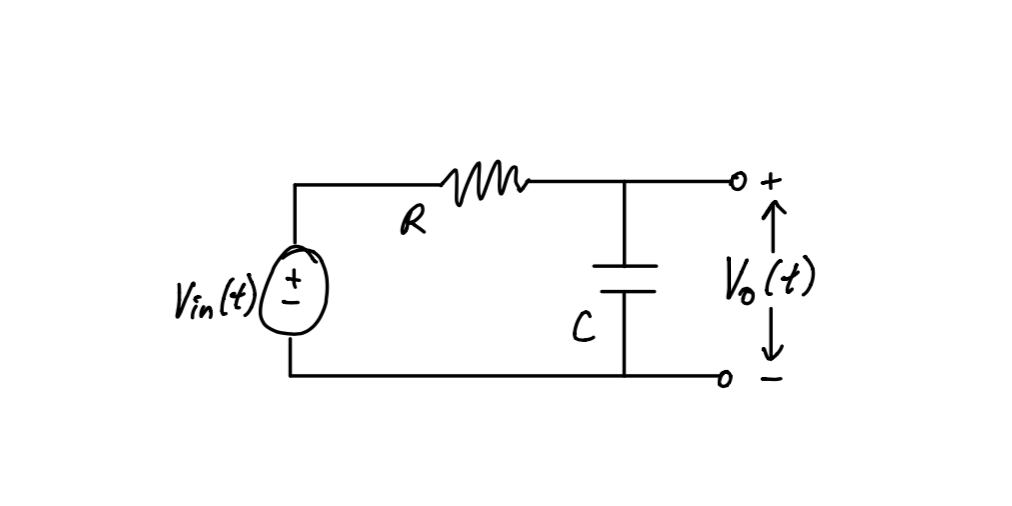
\includegraphics[scale=0.5]{RC.png}
\end{center}
\begin{equation}
\dot{V_0}(t)+\frac{V_0(t)}{RC}=\frac{V_{in}(t)}{RC}
\end{equation}
If this equation governs the time domain relationship between input and output, then its Fourier Transform should govern the frequency domain relationship! 
\begin{equation}
j\omega \hat{V}_0(\omega)+\frac{\hat{V}_0(\omega)}{RC}=\frac{\hat{V}_{in}(\omega)}{RC}
\end{equation}
Note that temporal derivative is represented in the frequency domain by multiplication by $j\omega$, you will prove this in a homework assignment. What we learned was that in the frequency domain the an LTI system is defined by $\hat{Y}(\omega)=\hat{H}(\omega)\hat{X}(\omega)$. Therefore, equation 4.9 can be manipulated to that form!
\begin{equation}
(j\omega RC +1)\hat{V}_0(\omega)=\hat{V}_{in}(\omega)
\end{equation}
\begin{equation}
\hat{V}_0(\omega)=\hat{V}_{in}(\omega)\frac{1}{(j\omega RC +1)}
\end{equation}
Therefore
\begin{equation}
\hat{H}(\omega)=\frac{1}{(j\omega RC +1)}
\end{equation}
We have found the Fourier Transform of the impulse response of the RC circuit! Why is this useful? If this $\hat{H}(\omega)$ is multiplied by $\hat{V}_{in}(\omega)$, it scales the frequency space of our input! Now in order to make physical sense of this multiplication it is necessary to manipulate the  complex expression for $\hat{H}(\omega)$ into polar form:
\begin{equation}
\hat{H}(\omega)=\frac{1}{(j\omega RC +1)}=\frac{1}{\sqrt{1+(\omega RC)^2}}e^{-j\tan^{-1}{(\omega RC)}}
\end{equation}
We can now see that the Fourier Transform of the input is multiplied by a magnitude and angle:
\begin{equation}
|\hat{H}(\omega)|=\frac{1}{\sqrt{1+(\omega RC)^2}} \: \: \: \: \: \& \: \: \: \: \: \angle \hat{H}(\omega) = -\tan^{-1}{(\omega RC)}
\end{equation}
This RC Circuit is called a continuous lowpass filter because as $\omega$ increases from $0$ to $\infty$, the magnitude of $\hat{H}(\omega)$ goes from 1 to 0. Since the magnitude of $\hat{H}(\omega)$ scales the Fourier Transform of the input, the input frequency space is \textit{filtered} by our RC circuit before reaching the output! We can use these types of circuits to manipulate the frequency content of continuous signals.\\

You will calculate the frequency response of a similar mechanical system in a homework assignment. 

\subsection{Bode Plots}
Bode plots represent 10 times the base 10 logarithm of the power of the frequency response of  filters on a log log scale. If you have some filter with frequency space representation $\hat{H}(\omega)$, then the bode plot of such a filter has $\log{(\omega)}$ on the x-axis and $20\log{| \hat{H}(\omega) |}$ on the y-axis. The multiplication by 20 instead of 10 is due to power being proportional to the square of voltage or current, and properties of the logarithm. \\

For example, we can show the bode plot of the lowpass RC filter from the last section as follows:
\begin{center}
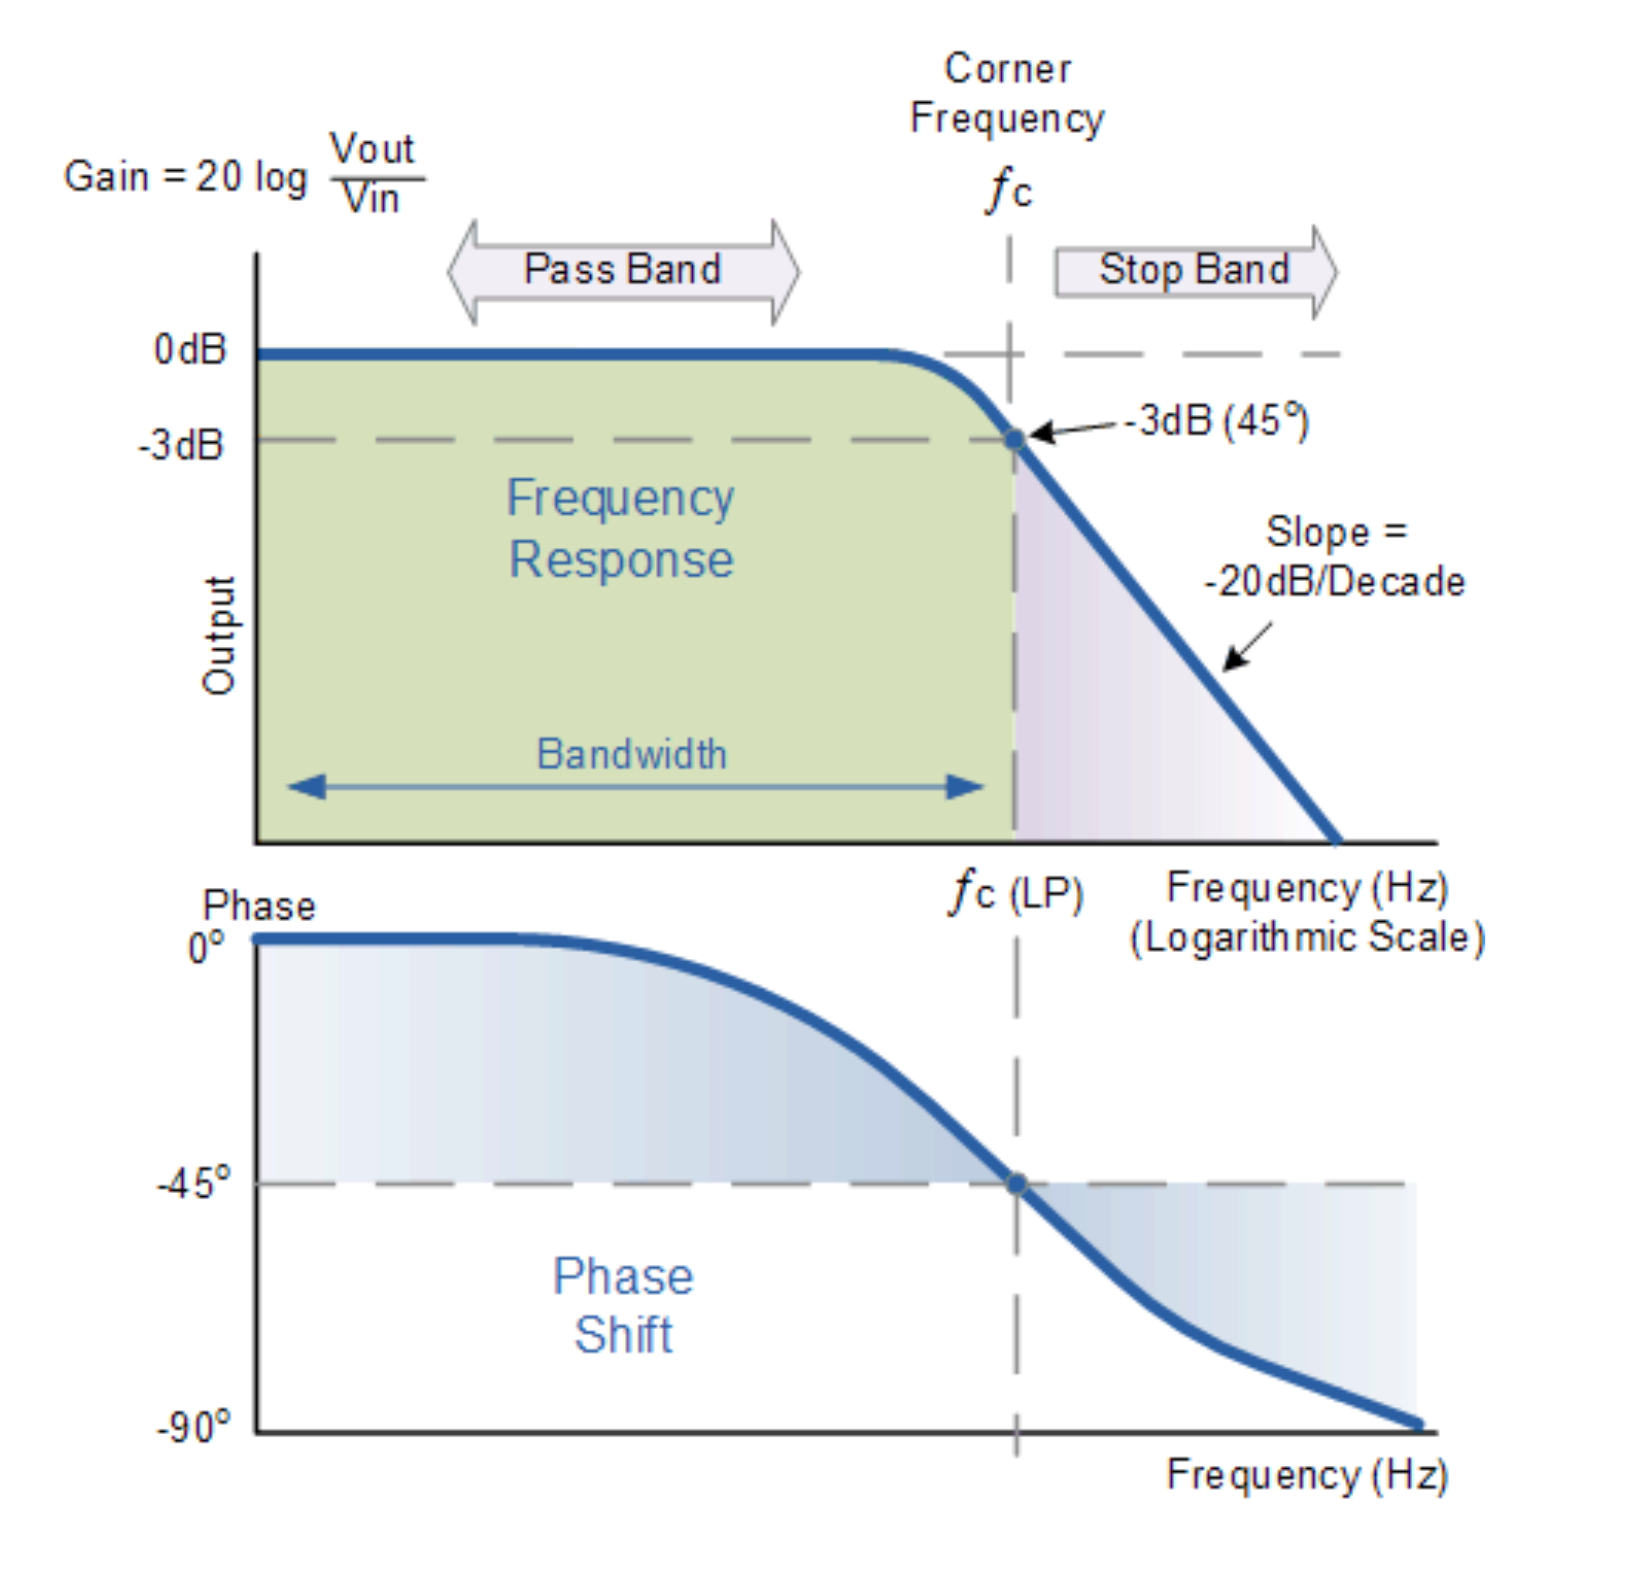
\includegraphics[scale=0.5]{bode.png}
\end{center}

The plot of the  $|\hat{H}(\omega)|$ is represented on the top and the plot of $\angle \hat{H}(\omega)$ is represented on the bottom. Note the phase plot is not on a log log scale. You can now clearly see why this particular circuit is a lowpass filter, (when multiplied by the Fourier Transform of the input, high frequency components are greatly attenuated). \\

The cutoff frequency $f_c$ is defined as the frequency at which the filter attenuates the power of an input signal by $\frac{1}{2}$. The rolloff rate is also important for filters and is defined as the slope of the stop band section of the bode plot on a log log scale.\\

Bode plots are an extremely common way of representing the frequency response of filters!

\section{Ideal Sampling}
Digital hardware operates in discrete steps, but the real world is analog, so we must have a way of converting continuous time signals into digital signals that computers can use. This process is known as sampling and we can model it mathematically as follows:\\

Suppose we have a continuous time signal $y(t)$ that is sampled every T seconds, we can represent that sampled signal as $y(nT)$ for integer valued $n$. The process is also represented by the following diagram. 

\begin{center}
\begin{tikzpicture}[auto, node distance=2cm,>=latex']
    \node [input, name=input](input) {$x[n]$};
    \node [block, right of=input] (sum) {Sampler};
    \node [output, name=output, right of=sum](output) {$y[n]$};
    \draw [blue,->, text=black](input) -- node{$y(t)$}(sum);
    \draw [blue,->,text=black] (sum) -- node {$y(nT)$} (output);
\end{tikzpicture}
\end{center}

A visual representation of this process is included below:
\begin{center}
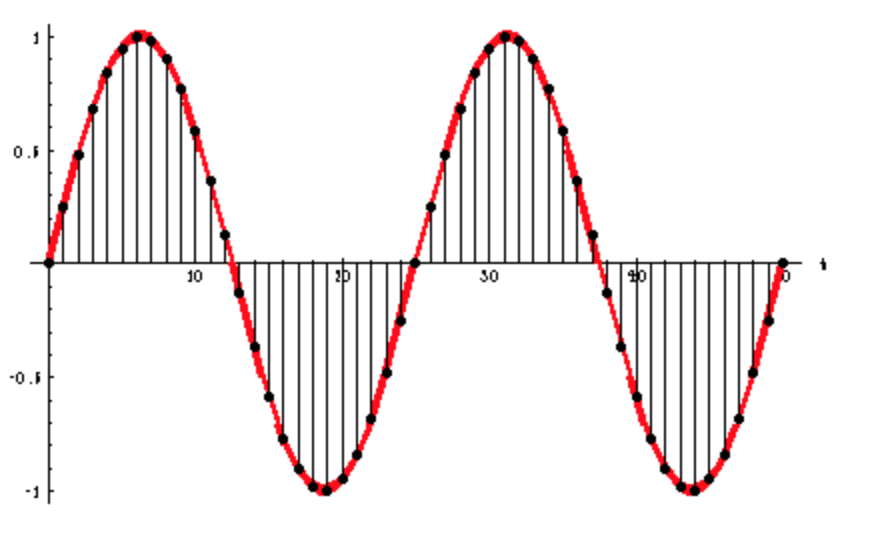
\includegraphics[scale=0.7]{example_sample.png}
\end{center}
The samples of the red sinusoid are represented as the black lines.
Although sampling seems like a seemingly painless process, we will explore the unapparent complexity and problems with the process.

\subsection{Aliasing}
Suppose we have a sinusoidal continuous signal of frequency $f$ that we would like to sample every $T$ seconds. 
\begin{equation}
y(t) \rightarrow y(nT)
\end{equation}
\begin{equation}
\sin(2\pi f t) \rightarrow \sin(2\pi f nT)
\end{equation}
Now what if we would like to sample a signal at a frequency $f+M/T$ every $T$ seconds, where $M$ is an integer. 
\begin{equation}
y(t) \rightarrow y(nT)
\end{equation}
\begin{equation}
\sin(2\pi (f+\frac{M}{T}) t) \rightarrow \sin(2\pi (f+\frac{M}{T}) nT)
\end{equation}
\begin{equation}
= \sin(2\pi f nT+2\pi \frac{M}{T} nT)
\end{equation}
\begin{equation}
= \sin(2\pi f nT+2\pi nM)
\end{equation}
\begin{equation}
= \sin(2\pi f nT)
\end{equation}
As you can see from equations 5.2 and 5.7, the two sampled signals look exactly the same! Therefore, we can ascertain that any signal with any two signals with a difference in frequency of $M/T$ will look exactly the same to our sampler! This phenomenon is called \textbf{aliasing}, and is a huge problem when it comes to sampling continuous signals from the physical world.\\

A visual representation of this phenomenon is included below:
\begin{center}
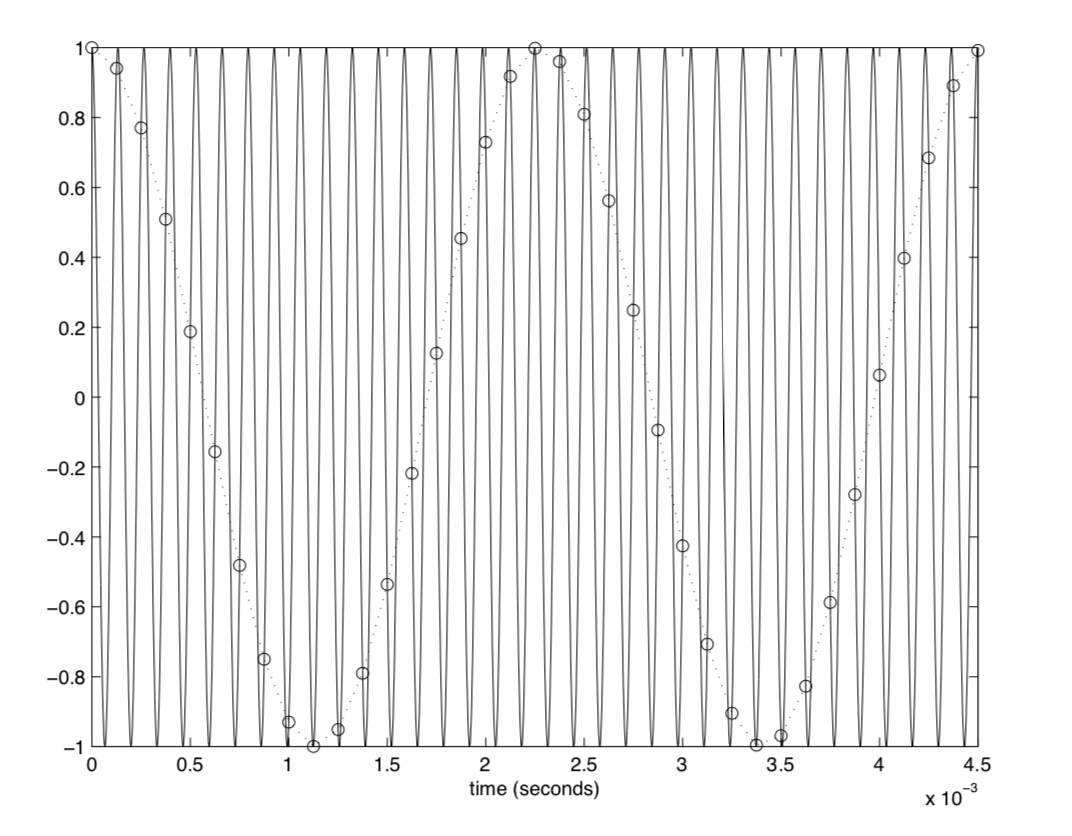
\includegraphics[scale=0.5]{sampled.png}
\end{center}
The continuous high frequency sinusoid is sampled at every small circle, and the small circles trace out a very different frequency signal than our continuous time signal!

\subsection{Analog to Digital}
We can use the Fourier Transform machinery we've developed to analyze the process of sampling much more formally. \\

The process of sampling a continuous time signal can be mathematically represented by multiplying the input signal by a periodic pulse train (periodic train of delta functions). For example, given an input signal $x(t)$, sample period T,  and sampled signal $y(t)$:
\begin{equation}
y(t)=x(t)\sum_{n=-\infty}^{\infty}\delta(t-nT)
\end{equation}
\begin{equation}
y(t)=\sum_{n=-\infty}^{\infty}x(nT)\delta(t-nT)
\end{equation}
We see that our sampled signal is represented by a sequence of weighted delta functions. This abstraction allows for the construction of individually valued points from our continuously valued input. \\

We have learned that convolution in time corresponds to multiplication in frequency, \textit{and} that multiplication in time corresponds to convolution in frequency (although this was not proven). 
\begin{equation}
f(t)g(t) \Longleftrightarrow \frac{1}{2\pi} \hat{f}(\omega)*\hat{g}(\omega)
\end{equation}

So how can we represent the frequency space, $\hat{f}(\omega)$, of our sampled signal $y(t)$? First, we must find the Fourier Transform of a pulse train.\\

\textbf{It is important to note that the easiest way to find the Fourier Transform of a period function is through its Fourier Series representation}. The Fourier Transform of a pulse train periodic in T is calculated as follows:\\

We first find the Fourier Series coefficients $a_n$. 
\begin{equation}
a_n = \frac{1}{T}\int_{-T/2}^{T/2}dt\: \delta (t) e^{-j 2 \pi n t /T} = \frac{1}{T}
\end{equation}
*An interactive plot of the reconstruction of the periodic delta function can be found \href{https://www.desmos.com/calculator/jcrawlfvwc}{here}.\\

\textbf{We need to find the Fourier transform that gives the same result as the Fourier series.}
Now since the inverse fourier \textbf{series} is of the following form:
\begin{equation}
f(t)=\sum_{k=-\infty}^{\infty}c_k e^{j2\pi kt/T}
\end{equation}
And the inverse fourier \textbf{transform} is of the following form:
\begin{equation}
f(t)=\frac{1}{2\pi}\int_{-\infty}^{\infty} d\omega \; \hat{f}(\omega) e^{j\omega t}
\end{equation}
$\hat{f}(\omega)$ must take the following form in order to get the same $f(t)$:
\begin{equation}
\hat{f}(\omega)=\frac{2\pi}{T}\sum_{k=-\infty}^{\infty}\delta(\omega-\frac{2\pi k}{T})
\end{equation}
Working through the math to show the desired result:
\begin{equation}
f(t)=\frac{1}{2\pi}\int_{-\infty}^{\infty} d\omega \; \hat{f}(\omega) e^{j\omega t}
\end{equation}
\begin{equation}
f(t)=\frac{1}{2\pi}\int_{-\infty}^{\infty} d\omega \; \frac{2\pi}{T}\sum_{k=-\infty}^{\infty}\delta(\omega-\frac{2\pi k}{T}) e^{j\omega t}
\end{equation}
\begin{equation}
f(t)=\frac{1}{T}\sum_{k=-\infty}^{\infty}\int_{-\infty}^{\infty} d\omega \; \delta(\omega-\frac{2\pi k}{T}) e^{j\omega t}
\end{equation}
\begin{equation}
f(t)=\frac{1}{T}\sum_{k=-\infty}^{\infty}e^{j2\pi k t/T}
\end{equation}
Where we can clearly see that $c_n$ is equal to $1/T$ as expected.\\

Now that we know the Fourier transform of our sampling signal (the periodic pulse train), we can find the Fourier transform of our sampled signal $\hat{y}(\omega)$ by convolution:
\begin{equation}
\hat{y}(\omega) = \frac{1}{2\pi}\hat{x}(\omega) * \frac{2\pi}{T}\sum_{k=-\infty}^{\infty}\delta(\omega-\frac{2\pi k}{T})
\end{equation}
\begin{equation}
\hat{y}(\omega) = \frac{1}{T}\int_{-\infty}^{\infty}d\omega' \: \sum_{k=-\infty}^{\infty}\delta(\omega'-\frac{2\pi k}{T})\hat{x}(\omega-\omega')
\end{equation}
\begin{equation}
\hat{y}(\omega) = \frac{1}{T}\sum_{k=-\infty}^{\infty}\int_{-\infty}^{\infty}d\omega' \: \delta(\omega'-\frac{2\pi k}{T})\hat{x}(\omega-\omega')
\end{equation}
\begin{equation}
\hat{y}(\omega) = \frac{1}{T}\sum_{k=-\infty}^{\infty}\hat{x}(\omega-\frac{2\pi k}{T})
\end{equation}
If we define our sampling angular frequency as $\omega_s = 2\pi / T $, the the equation becomes:
\begin{equation}
\hat{y}(\omega) = \frac{1}{T}\sum_{k=-\infty}^{\infty}\hat{x}(\omega-\omega_s k)
\end{equation}
We can see that the Fourier transform of our sampled continuous function is equal to a sum of scaled and shifted copies of our original input signal's Fourier transform, and the period of $\hat{y}(\omega)$ is our sampling frequency $\omega_s$! The process is represented visually below:
\begin{center}
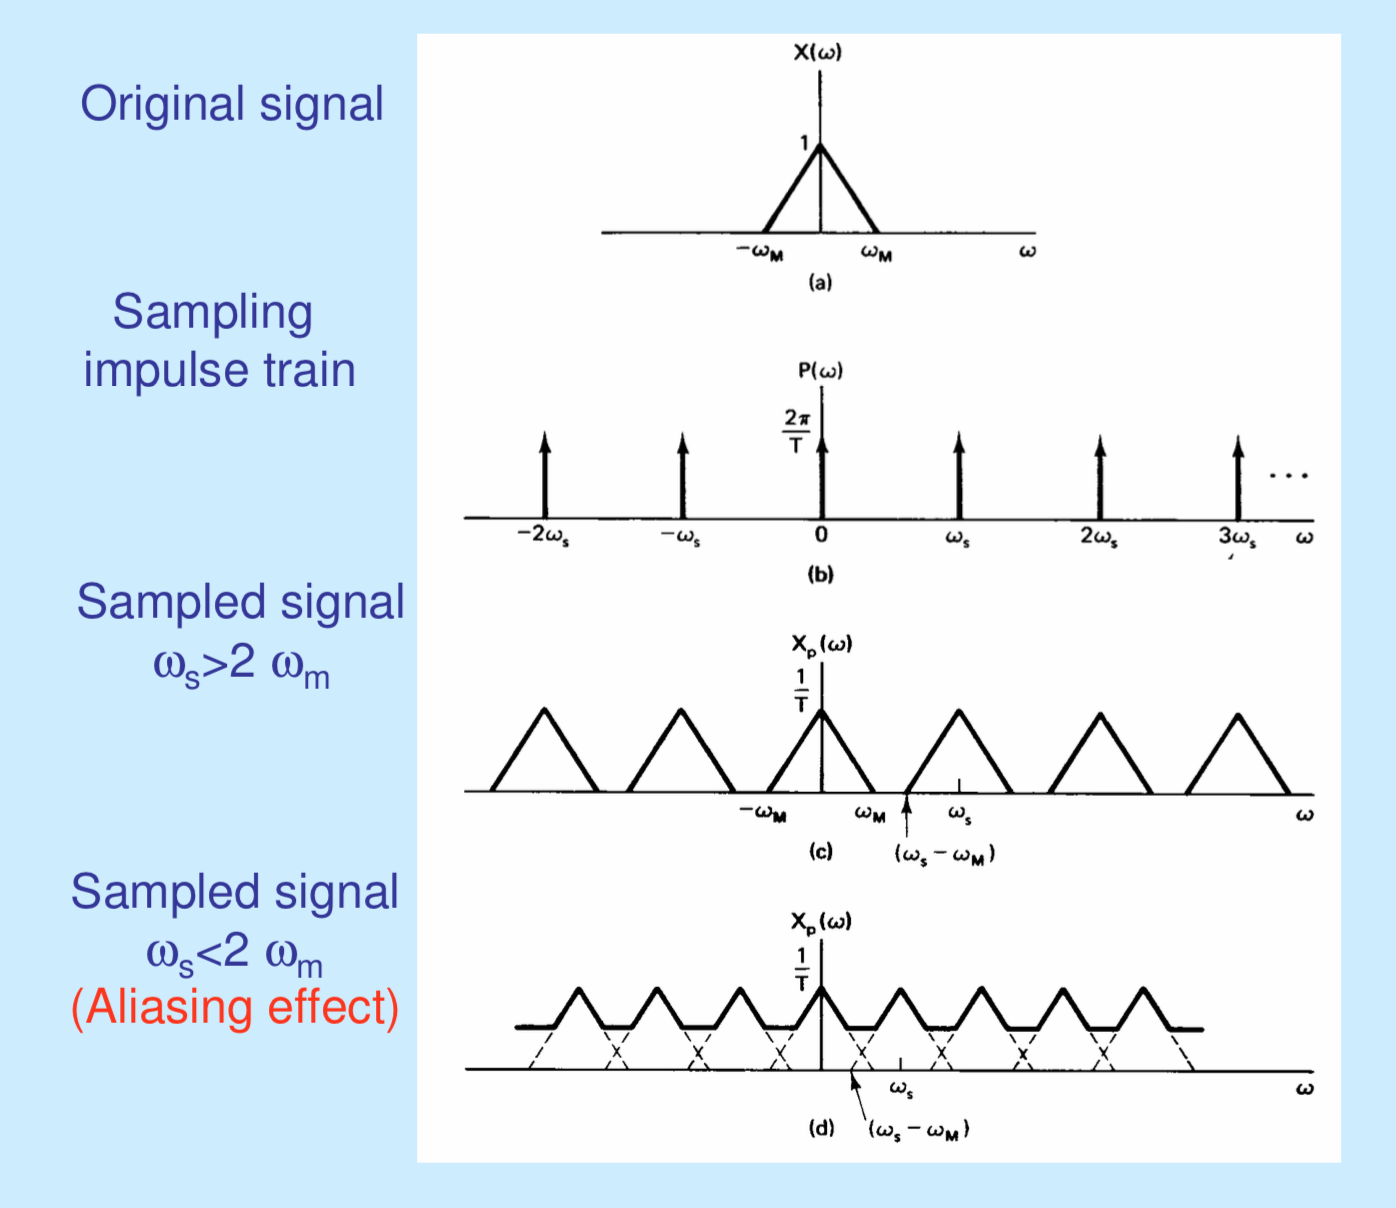
\includegraphics[scale=0.5]{aliasing.png}
\end{center}

*The overlap in the in the fourth plot is the negative effect produced by the aliasing discussed in section 5.1. This will be analyzed further soon. \\

Now we have only discussed the continuous time representation of our sampling system, but we are trying to construct discrete signals.
We said that sampling is of a continuous time signal was represented by the following:
\begin{equation}
y(t) \rightarrow x(nT)
\end{equation}
Remember that $x$ is just sampled $y$, therefore $x(nT)$ is basically a discrete signal $x[n]$.
\begin{equation}
y(t) \rightarrow y(nT) \rightarrow x(nT) \rightarrow x[n]
\end{equation}
This process is abstracted away into a ADC (Analog to Digital Converter).
\begin{center}
\begin{tikzpicture}[auto, node distance=2cm,>=latex']
    \node [input, name=input](input) {$x[n]$};
    \node [block, right of=input] (sum) {ADC};
    \node [output, name=output, right of=sum](output) {$y[n]$};
    \draw [blue,->, text=black](input) -- node{$x(nT)$}(sum);
    \draw [blue,->,text=black] (sum) -- node {$x[n]$} (output);
\end{tikzpicture}
\end{center}
***Note that we have already shown that the DTFT is periodic every $\Omega=2\pi$. So it makes sense that the CFT of our sampled signal is periodic in exactly the same thing (the units of $\Omega$ are radians per sample, and the definition of $\omega_s$ is angular sampling frequency)! Also note that \textbf{the units of $\Omega$ is radians/sample}, and \textbf{the units of $\omega_s$ is radians/second}. ****\textbf{In conclusion, the CFT of our sampled signal is the DTFT of that discrete signal} (up to a scale factor).****\\

Now if we are analyzing the frequency content of the newly constructed discrete signal, based on the above image, it is clear that any frequency content of our original signal that overlaps with the sequential copies is no longer the same frequency content in the DTFT. Therefore, our sampling process will map higher frequency content to lower frequencies which are not actually present. This consequence is the reason why \textbf{we must not have any frequency content in our original signal greater than half of our sampling frequency}! The minimum sampling rate in order to capture all of the frequency content of a signal accurately is known as the \textbf{Nyquist Rate}, and the maximum frequency that can be accurately described by a sampled signal is known as the \textbf{Nyquist Frequency},


\subsection{Digital to Analog}
Now what if we want to convert our digital signal back into the original continuous signal? We must first convert our digital $x[n]$ back into a continuous function. This process can be abstracted away into some ADC (Analog to Digital Converter). \textbf{Think of this as recreating the scaled pulse train produced at the beginning of the sampling process}. 

\begin{center}
\begin{tikzpicture}[auto, node distance=2cm,>=latex']
    \node [input, name=input](input) {$x[n]$};
    \node [block, right of=input] (sum) {ADC};
    \node [output, name=output, right of=sum](output) {$y[n]$};
    \draw [blue,->, text=black](input) -- node{$x[n]$}(sum);
    \draw [blue,->,text=black] (sum) -- node {$x(nT)$} (output);
\end{tikzpicture}
\end{center}

 We know the frequency space representation of our input, and the frequency space representation of our sampled signal, so why not apply a filter to our sampled signal that will recover our original signal!\\

We can apply an ideal bandpass filter to our sampled signal and reconstruct our original signal as shown below:

\begin{center}
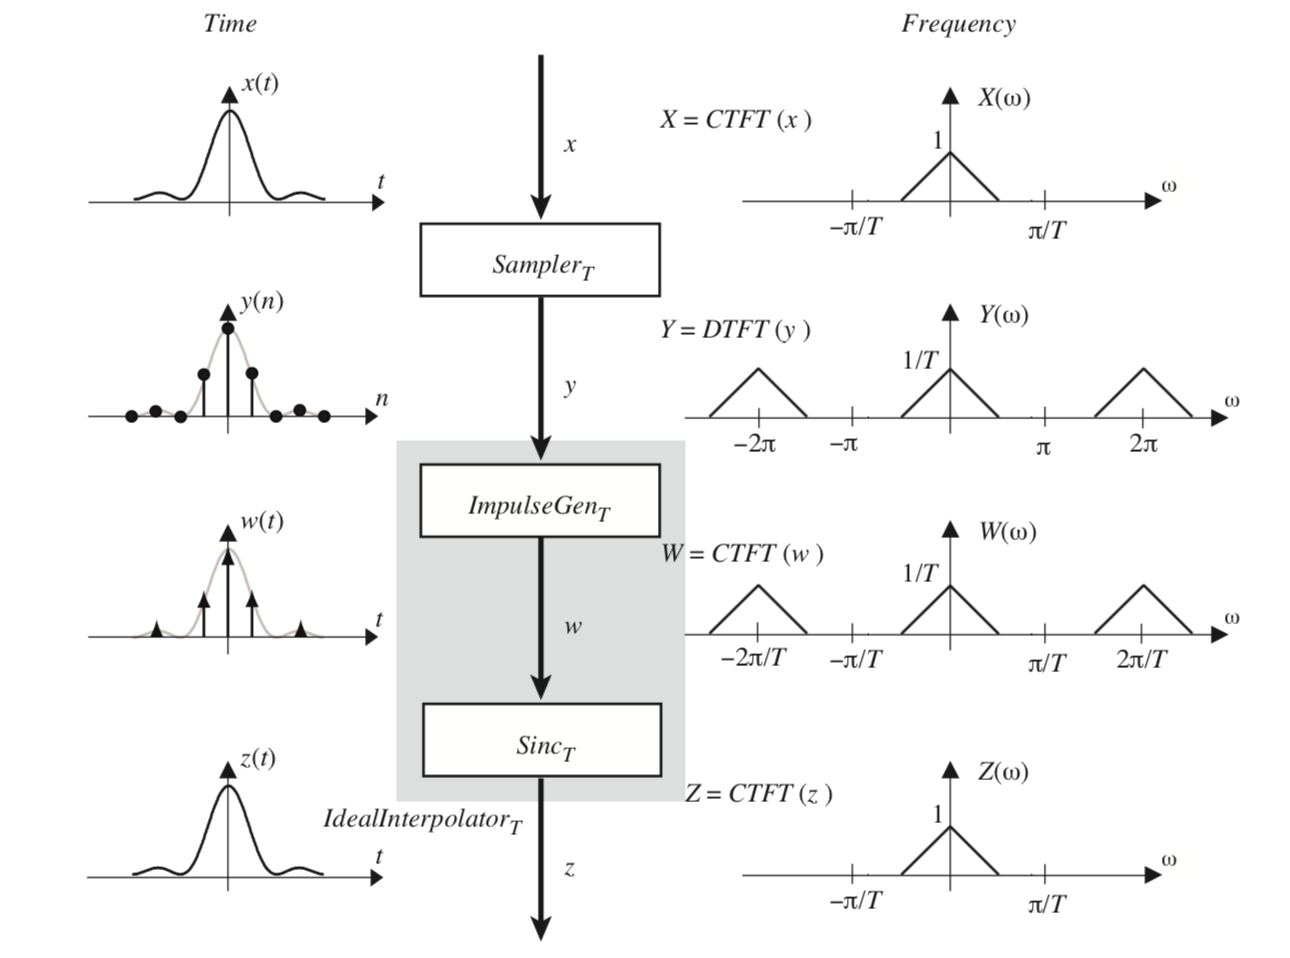
\includegraphics[scale=0.7]{reconstruct.png}
\end{center}

The band pass filter must have the following equation:
\begin{equation}
h(\omega) \equiv
\begin{cases} 
      T & |\omega| < \omega_s/2=\pi/T \\
      0 & \text{else}
\end{cases}
\end{equation}

The temporal representation of this ideal bandpass filter can be calculated to be a continuous sinc function scaled by $T$.
\begin{equation}
h(t)=\frac{T}{2\pi}\int_{-\frac{\omega_s}{2}}^{\frac{\omega_s}{2}}d\omega \; e^{j\omega t}
\end{equation}
\begin{equation}
h(t)=\frac{T}{j2\pi n }\big[ e^{j\omega t}\big]_{-\frac{\omega_s}{2}}^{\frac{\omega_s}{2}}
\end{equation}
\begin{equation}
h(t)=\frac{T}{j2\pi t }\big( e^{j\frac{\omega_s}{2} t}-e^{-j\frac{\omega_s}{2} t}\big)
\end{equation}
\begin{equation}
h(t)=\frac{T2j\sin{(\frac{\omega_s}{2} t)}}{j2\pi t }
\end{equation}
\begin{equation}
h(t)=\frac{T\sin{(\frac{\omega_s}{2} t)}}{\pi t }
\end{equation}

We have shown how to perfectly reconstruct our sampled signal.

*Note, to apply this filter in the time domain we must convolve our sampled signal with h(t), a function with infinite range! This is one of the reasons why, in practice, ideal reconstruction is difficult to implement and other methods are used (interpolation, zero-order hold, etc). You can read about interpolation \href{https://en.wikipedia.org/wiki/Interpolation}{here}, and zero-order hold \href{https://en.wikipedia.org/wiki/Zero-order_hold}{here}.


\section{Laplace \& Z-Transforms, Feedback Control}
\subsection{Introduction}
We will now analyze generalizations of the Fourier Transform and Discrete Time Fourier Transform. These new tools are extremely useful for system analysis and predicting system stability. 

\subsubsection{Laplace Transform}
The Laplace transform is another way of representing continuous functions. We can think of it as taking the $j\omega$ from the exponent of the Fourier Transform and generalizing it to a new value $s=\sigma +j\omega$ with both real and imaginary values. We define the Laplace transform as follows:
\begin{equation}\boxed{
F(s)=\int_{0^-}^{\infty}dt\; f(t)e^{-st}}
\end{equation}
The integral only starts at $t=0^{-}$ to because we are now focusing of system analysis, in which are our signals can be made to start at $t=0$. \textbf{Notice that since $s=\sigma +j\omega$ we can find the Laplace transform for functions which we could not find the Fourier transform (unbounded at $\infty$), as long as the exponential $e^{-st}$ decays faster than $f(t)$ grows!} \\

It can be shown using the techniques of Complex Analysis that the inverse Laplace Transform is the following:
\begin{equation}\boxed{
f(t) = \frac{1}{2\pi j}\lim_{T\rightarrow \infty}\int_{\gamma-jT}^{\gamma+jT} ds\: F(s) e^{st}}
\end{equation}

\textbf{A Couple Useful Properties:}\\
\textit{time-shift} (prove as HW):
\begin{equation}
F(t-t_0)=e^{-st_0}F(t)
\end{equation}
\textit{temporal derivatives}:
\begin{equation}
F(s)=\int_{0^-}^{\infty} dt\; f^{(n)}(t)e^{-st}
\end{equation}
Use integration by parts multiple times:
\begin{equation}
F(s)=f^{(n-1)}(t)e^{-st}\Big|_{0^-}^{\infty}+s\int_{0^-}^{\infty} dt\; f^{(n-1)}(t)e^{-st}
\end{equation}
\begin{equation}
F(s)=f^{(n-1)}(\infty)e^{-s\infty}-f^{(n-1)}(0^-)+s\int_{0^-}^{\infty} dt\; f^{(n-1)}(t)e^{-st}
\end{equation}
Where the $t=\infty$ term must equal zero for the Laplace transform to exist.
\begin{equation}
F(s)=-f^{(n-1)}(0^-)+s\int_{0^-}^{\infty} dt\; f^{(n-1)}(t)e^{-st}
\end{equation}
In general, we can express the time derivative in the Laplace domain as follows:
\begin{equation}
\mathcal{L}\{f'\}=sF(s)-f(0^-)
\end{equation}
\begin{equation}
\mathcal{L}\{f''\}=s^2F(s)-sf(0^-)-f'(0-)
\end{equation}
\begin{equation}
\mathcal{L}\{f^{(n)}\}=s^nF(s)-s^{n-1}f(0^-)-s^{n-2}f'(0^-)-...-f^{(n-1)}(0^-)
\end{equation}
Where $\mathcal{L}(f)$ denotes the Laplace transform.

\textbf{Examples:}\\
What is the Laplace transform of $e^{at}$? 
\begin{equation}
F(s)=\int_{0^-}^{\infty}dt\; e^{at}e^{-st}
\end{equation}
\begin{equation}
F(s)=\int_{0^-}^{\infty}dt\; e^{(a-s)t}
\end{equation}
Note that this integral will only converge if $\Re(a-s)$ is less than 0.
\begin{equation}
F(s)=\frac{1}{a-s}\big[ e^{(a-s)t} \big]_{0^-}^{\infty}
\end{equation}
\begin{equation}
F(s)=\frac{1}{a-s}\big[ e^{(a-s)t} \big]_{0^-}^{\infty} = \frac{1}{a-s}
\end{equation}

Find the Laplace transform of $t e^{at}$ as HW. How would you find the Laplace transform of $\sin{(at)}$ or $\cos{(at)}$?

\textbf{Region of Convergence:}\\
In the previous examples the Laplace transform of $e^{at}$ only converged if $\Re(a-s)$ was less than 0. We will call the range of $s$ for which the Laplace transform is non-infinite the \textbf{region of convergence}.\\

Taking $\Re(a)$ to be a positive number, the region of convergence of the Laplace transform of $e^{at}$ is the following:

\begin{center}
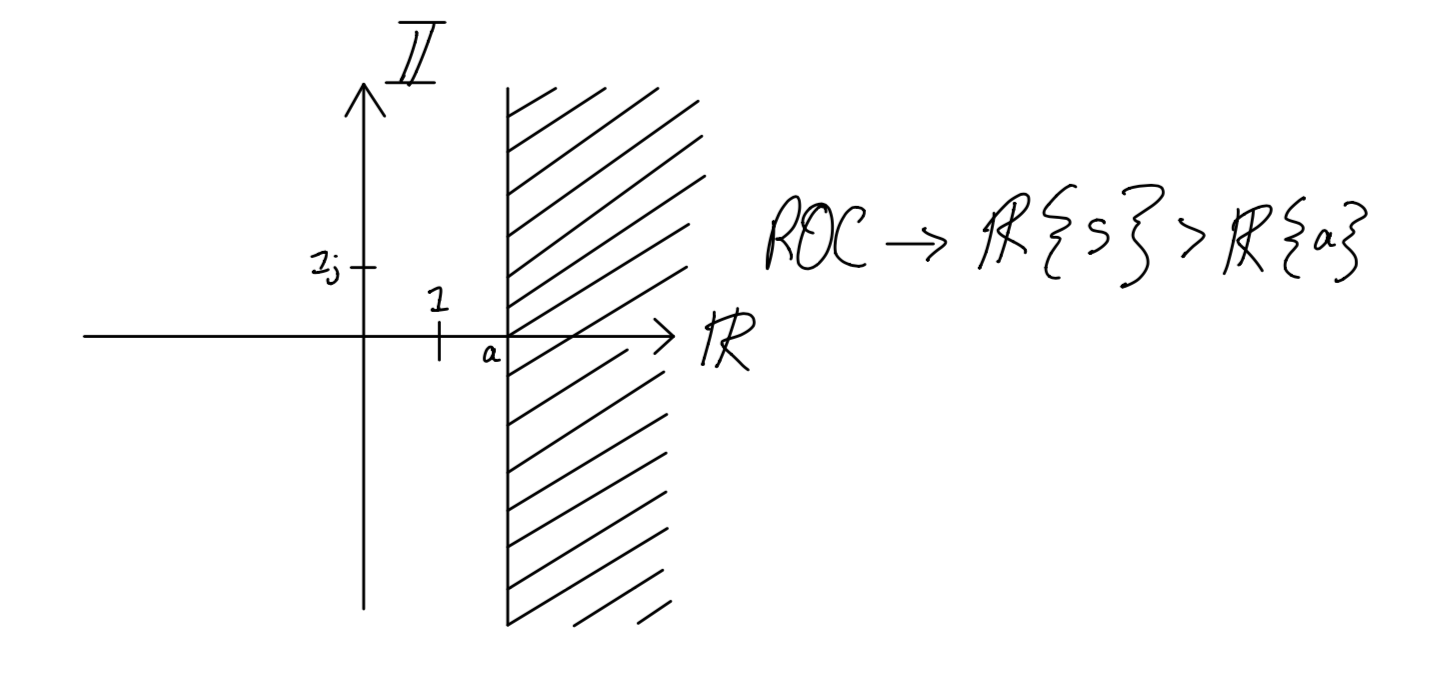
\includegraphics[scale=0.65]{S_convergence.png}
\end{center}

\subsubsection{Z Transform}
The Z transform is another way of representing Discrete signals (which will result in the familiar operator notation from section 1). We define the Z transform as follows:
\begin{equation}\boxed{
X(z)=\sum_{n=-\infty}^{\infty} x[n]z^{-n}}
\end{equation}
Where $z$ is a complex number. This is similar to the DTFT if we think of $z$ as a replacement for $e^{-j\Omega}$. \\

It can be shown using the techniques of Complex Analysis that the inverse Z Transform is the following:
\begin{equation}\boxed{
f(t) = \frac{1}{2\pi j}\oint_{C} dz\: X(z) z^{n-1}}
\end{equation}

\textbf{Useful Properties:}\\

\textit{n-shift} (prove as HW):
\begin{equation}
\mathcal{Z}\{x[n-n_0]\}=z^{-n_0} X(z)
\end{equation}
Where $\mathcal{Z}(x)$ denotes the Z transform.

\textbf{Examples:}\\
What is the Z transform of $x[n]=a^{n}u[n]$?

\begin{equation}
X(z)=\sum_{n=-\infty}^{\infty} a^{n}u[n] z^{-n}
\end{equation}
\begin{equation}
X(z)=\sum_{n=0}^{\infty} a^{n}z^{-n}=\sum_{n=0}^{\infty} \Big(\frac{a}{z}\Big)^{n}
\end{equation}
Note that this sum will only converge if $|\frac{a}{z}|$ is less than 1.
\begin{equation}
X(z)=\frac{1}{1-a/z}=\frac{1}{1-az^{-1}}=\frac{z}{z-a}
\end{equation}
Does this look like the discrete time transfer function of any familiar LTI system?

\textbf{Region of Convergence:}\\
The values for which the Z transform of a discrete time signal converge are enclosed in the \textbf{region of convergence} of the Z transform. \\

Taking $|a|$ to be less than 1, the region of convergence of the Z transform of $a^{n}$ is the following:

\begin{center}
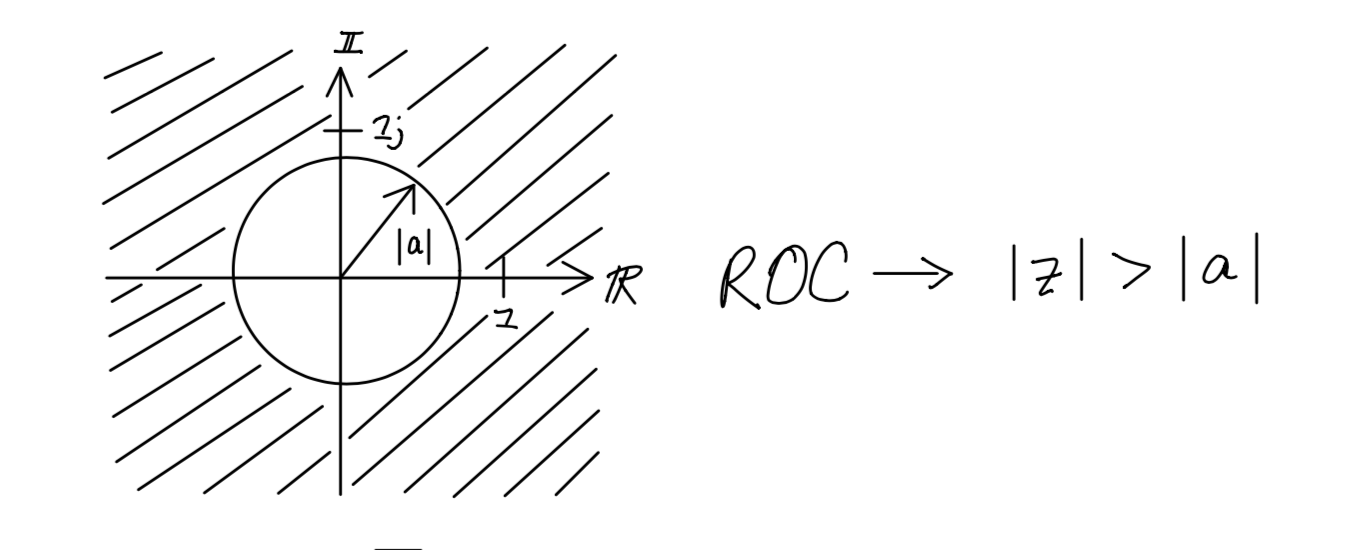
\includegraphics[scale=0.65]{Z_convergence.png}
\end{center}

\subsection{Convolution \& Multiplication}
\subsubsection{Continuous}
It can be shown that convolution in the temporal domain corresponds to multiplication in the frequency domain of the Laplace transform as follows.
\begin{equation}
h(t) =  f(t)*g(t)
\end{equation}
\begin{equation}
h(t) =  \int_{0^-}^{\infty}dt_1\; f(t_1) g(t-t_1)
\end{equation}
Taking the Laplace transform of both sides (using the shift property)
\begin{equation}
H(s) =  \int_{0^-}^{\infty}dt_1\; f(t_1) e^{-t_1s}G(s)
\end{equation}
\begin{equation}
H(s) =  F(s)G(s)
\end{equation}



\subsubsection{Discrete}
It can be shown that convolution in the temporal domain corresponds to multiplication in the frequency domain of the Z transform as follows.  
\begin{equation}
h[n]=f[n]*g[n] = \sum_{k=\infty}^{\infty}f[k]g[n-k]
\end{equation}
We now take the Z transform of both sides using the superposition and delay property:
\begin{equation}
H(z)=\sum_{k=\infty}^{\infty}f[k]z^{-k}G(z)
\end{equation}
\begin{equation}
H(z)=F(z)G(z)
\end{equation}
Now if we think back to discrete LTI systems, this is exactly what we were doing with the operator notation! We simply rename variables as follows and we can immediately recognize $X$ as our input signal, $H$ as our system functional, and $Y$ as our output!

\begin{center}
\begin{tikzpicture}[auto, node distance=2cm,>=latex']
    \node [input, name=input](input) {$X$};
    \node [block, right of=input] (sum) {$H$};
    \node [output, name=output, right of=sum](output) {$Y$};
    \draw [blue,->, text=black](input) -- node{$X$}(sum);
    \draw [blue,->,text=black] (sum) -- node {$Y$} (output);
\end{tikzpicture}
\end{center}

\begin{equation}
Y(z)=H(z)X(z)
\end{equation}
We simply didn't explicitly calculate $Y(z)$ and $X(z)$ because they are dependent on unknown input. 

\subsection{Application to LTI Systems}
Now that we've been introduced to the Laplace and Z transforms, a couple of their useful properties, and the fact their relationship with convolution/multiplication a clear connection to LTI systems should be apparent. We've already discussed using the Fourier transform to find solutions to LTI systems, but we now have an even more generalized and powerful tool that can be directly related to our algebraic expressions for discrete time systems as well as handle unbounded functions. 

\subsubsection{Discrete Time Systems}
If you look back to section 1.1, it should be clear to you that taking the Z transform of a discrete LTI system (starting with the functional representation) corresponds to writing the LTI system in what we called "operator" notation. A brief reminder of this process:
\begin{equation}
y[n]=ax[n]-by[n-1]
\end{equation}
Taking the Z transform of both sides (using time shift property and linearity):
\begin{equation}
Y(z)=aX(z)-bz^{-1}Y(z)
\end{equation}
We have learned that we can find the output of LTI systems using the convolution of the input with the unit sample response, we have also learned that convolution in the sample domain corresponds to multiplication in the Z domain, therefore the product of $X(z)$ with some function $H(z)$ must equal to $Y(z)$. 
\begin{equation}
Y(z)+bz^{-1}Y(z)=aX(z)
\end{equation}
\begin{equation}
(1+bz^{-1})Y(z)=aX(z)
\end{equation}
\begin{equation}
\frac{Y(z)}{X(z)}=H(z)=\frac{a}{1+bz^{-1}}
\end{equation}
\textbf{Importantly, $H(z)$ must equal the Z transform of the unit sample response of this system!} We can use the Z transform to solve for the unit sample response of any LTI system using the following technique. \\

\textbf{Finding Impulse Response:}\\

\textbf{1:}  Find the system functional representation of any LTI system given in general form (where for brevity we will denote the Z transform of a signal $f[n]$ as $F$):
\begin{equation}
H=\frac{Y}{X}=\frac{\sum_{j=0}^{n} b_j z^{-j}}{\sum_{i=0}^{m} a_i z^{-i}}
\end{equation}
\textbf{2:}  By the fundamental theorem of algebra, any order $n$ polynomial has $n$ complex roots (counted with multiplicity). With this in mind, we can rewrite any transfer function in the following form:
\begin{equation}
H=\frac{Y}{X}=\frac{\prod_{j=0}^{n} (1-c_j z^{-1})}{\prod_{i=0}^{m}(1-d_i z^{-1})}
\end{equation}
*The values of $z$ for which the numerator is 0, $(c_j)$, are known as the \textbf{zeros} of the transfer function, and the values of $z$ for which the denominator is 0, $(d_i)$, are known as the \textbf{poles} of the transfer function. 

\textbf{3:}  Decompose the denominator of the previous expression into a sum using partial fraction decomposition.
\begin{equation}
H=\frac{Y}{X}=\prod_{j=0}^{n} (1-c_j z^{-1})\sum_{i=0}^{m}\frac{A_i}{1-d_i z^{-1}}
\end{equation}
\textbf{4:}  In general, this sum of fractions can be inverted to the time domain representation using a variety of techniques (z transform table, analytical), but for our simple functions the following method will suffice (although it will \textbf{NOT} always work, due to complexities with repeated roots and non-exponential functions):\\

Note that a z transform of the form:
\begin{equation}
H_i(z)=\frac{a_i z^{-n_0}}{1-d_i z^{-1}}
\end{equation}
corresponds to the following discrete function (since the time shift and linearity tell us how to handle the numerator). The $z^{-n_0}$ delays the function by $n_0$ and the $a_i$ is simply a scale factor.
\begin{equation}
h_i[n] = a_i d_i^{n-n_0}
\end{equation}
So following partial fraction decomposition, and taking advantage of the linearity of the Z transform, we can clearly see that after multiplying out the numerator of expression 6.37, the impulse response $h[n]$ can be represented as a sum of scaled and shifted exponentials (that may be complex).

*I have also attached a table of inverse Z transforms to make your life easier (although light partial fraction decomposition may still be required in the homework).

\textbf{STABILITY:}\\
Note that now we have a well established method of solving for the impulse response of a discrete LTI system, we should be able to easily see whether or not the system is stable (does not tend towards $\pm \infty$, or oscillate forever). We have seen that each pole of the transfer function $(d_i)$ corresponds to the base of an exponential function (or a more complex function which we have not discussed) in the impulse response, so it should be clear that the impulse response will only be stable if the magnitude of all poles $(d_i)$ is less than 1. \\

For example: If the system we just solved above in equation 6.37 and 6.38, is the following:

\begin{equation}
H_i(z)=\frac{a_i z^{-n_0}}{1-d_i z^{-1}}  \Longleftrightarrow h_i[n] = a_i d_i^{n-n_0}
\end{equation}

We can clearly see that $h_i[n]$ will grow to infinity or oscillate forever unless $|d_i|$ is less than 1.

\textbf{NOTE:}  The region of convergence of the Z transform also tells us something useful about stability. Since the response of a system can be characterized by a sum of scaled and shifted exponential functions (as shown above), they will each contribute to the region of convergence, (actually the exponential with the largest magnitude base will govern the ROC. \textbf{Therefore, if the region of convergence contains the unit circle, the system is stable.} Convince yourself this is true. 

\subsubsection{Continuous Time Systems}
We can also analyze continuous time systems in the Laplace domain.  The time-shift, temporal derivative, and convolution/multiplication properties we've demonstrated have extremely useful implications when it comes to solving differential equations and finding the impulse response of continuous LTI systems.

We can start with the usual representation of a continuous time system as a ordinary linear time invariant differential equation:
\begin{equation}
y'(t) + cy(t)=dx(t)
\end{equation}
Taking the Laplace transform of both sides utilizing the time derivative rule explained above yields the following:
\begin{equation}
sY(s)-y(0^-)+cY(s)=dX(s)
\end{equation}
Forcing rest initial conditions allows us to manipulate the equation into the following form:
\begin{equation}
Y(s)=\frac{d}{s+c}X(s)
\end{equation}
Again, we've shown that multiplication in the Laplace domain corresponds to convolution in the frequency domain, so $X(s)$ must be multiplied by the Laplace transform $H(s)$ of the impulse response $h[n]$ of our continuous LTI system!
\begin{equation}
Y(s)=\frac{d}{s+c}X(s)=H(s)X(s)
\end{equation}
\begin{equation}
H(s)=\frac{d}{s+c}
\end{equation}

\textbf{Finding Impulse Response}\\

After taking the Laplace Transform of an ordinary LTI differential equation, given rest initial conditions, the quotient of output and the input is defined as the \textbf{continuous transfer function}.
\begin{equation}
\frac{Y(s)}{X(s)}=H(s)
\end{equation}
*Note: evaluating this continuous transfer function at $s=j\omega$ exposes the \textit{filtering} properties of the continuous system!\\

We can find the impulse response of an ordinary LTI differential equation in a very similar method to that of discrete LTI systems (assume rest initial conditions):

Given an ordinary LTI differential equation of the form:
\begin{equation}
\cdots a_2y''(t)+a_1y'(t)+a_0y(t)=b_0x(t)+b_1x'(t)+b_2x''(t) \cdots
\end{equation}

\textbf{1:}  Find the transfer function of any ordinary LTI differential equation in general form (where for brevity we will denote the Laplace transform of a function $f(t)$ as $F(s)$):
\begin{equation}
H(s)=\frac{Y(s)}{X(s)}=\frac{\sum_{j=0}^{n} b_j s^{j}}{\sum_{i=0}^{m} a_i s^{i}}
\end{equation}
\textbf{2:}  By the fundamental theorem of algebra, any order $n$ polynomial has $n$ complex roots (counted with multiplicity). With this in mind, we can rewrite any transfer function in the following form:
\begin{equation}
H(s)=\frac{Y(s)}{X(s)}=\frac{\prod_{j=0}^{n} (1-c_j s)}{\prod_{i=0}^{m}(1-d_i s)}
\end{equation}
*The values of $s$ for which the numerator is 0, $(c_j)^{-1}$, are known as the \textbf{zeros} of the transfer function, and the values of $s$ for which the denominator is 0, $(d_i)^{-1}$, are known as the \textbf{poles} of the transfer function. 

\textbf{3:}  Decompose the denominator of the previous expression into a sum using partial fraction decomposition.
\begin{equation}
H(s)=\frac{Y(s)}{X(s)}=\prod_{j=0}^{n} (1-c_j s)\sum_{i=0}^{m}\frac{A_i}{1-d_i s}
\end{equation}
\textbf{4:}  In general, this sum of fractions can be inverted to the time domain representation using a variety of techniques (Laplace transform table, analytical), but for our simple functions the following method will suffice (although it will \textbf{NOT} always work, due to complexities with repeated roots and non-exponential functions):\\

Note that a Laplace transform of the form:
\begin{equation}
H(s)=\frac{a_i}{d_i - s}
\end{equation}
corresponds to the following continuous function
\begin{equation}
h(t) = a_i e^{d_i t}
\end{equation}
So following partial fraction decomposition, and taking advantage of the linearity of the Laplace transform, we can find the impulse response by summing the contributions of multiple fractions. \textbf{You will not have to deal with finding the impulse response of functions involving the derivative of the input}

**Take advantage of the provided Laplace table when solving homework problems (although light partial fraction decomposition may still be required in the homework).


\textbf{Solving Ordinary LTI Differential Equations}

It is possible to completely solve many ordinary linear differential equations using the Laplace transform (they don't need to be time invariant) using the convolution/multiplication properties. You simply follow the same method as outlined for finding impulse response, but solve for $Y(s)$ instead of $Y(s)/X(s)$, (where $Y$ is output and $X$ is input).

\textbf{example:}

Solve $\dot{x}+3x=e^{-t}, x(0^-)=4$.\\

Start by taking the Laplace transform of both sides:
\begin{equation}
sX(s)-x(0^-)+3X(s)=\frac{1}{1+s}
\end{equation}
Plugging in initial conditions and solving for $X(s)$:
\begin{equation}
sX(s)+3X(s)=\frac{1}{1+s}+4
\end{equation}
\begin{equation}
X(s)(s+3)=\frac{1}{1+s}+4
\end{equation}
\begin{equation}
X(s)=\frac{1}{(1+s)(s+3)}+\frac{4}{s+3}
\end{equation}
We now need to perform partial fraction decomposition on the first term, yielding:
\begin{equation}
X(s)=\frac{1/2}{s+1}-\frac{1/2}{s+3}+\frac{4}{s+3}
\end{equation}
\begin{equation}
X(s)=\frac{1/2}{s+1}+\frac{7/2}{s+3}
\end{equation}
And finally looking up inverse Laplace relationship:
\begin{equation}
x(t)=\frac{e^{-t}}{2}+\frac{7e^{-3t}}{2}
\end{equation}
Which satisfies the given differential equation and initial conditions. 


\section{Basic Signal Modulation}
Signal modulation is a very useful method of transmitting information over mediums which they might not traverse well in their base form. AM (amplitude modulation) and FM (frequency modulation) radio are great examples of modulating signals to transmit audio signals over great distances. We will explore the basic characteristics of a few simple modulation schemes, and leave the detailed implementation and more complex schemes to higher level courses. 

\subsection{Amplitude Modulation}
Amplitude modulation, as the name states, is the method of modulating the amplitude of some high frequency \textit{carrier wave} with the information to be transmitted. As we well know, the information to be transmitted can be deconstructed into a sum of weighted harmonic waves with a certain bandwidth (width of frequency space representation). We will explore amplitude modulation of the following form:\\

Suppose the information we want to transmit is some signal $f(t)$, with Fourier transform $\hat{F}(\omega)$ with a restricted bandwidth $B$  and center frequency $\omega_0$ (note, real signals will exhibit frequencies around $-\omega_0$ as well):
\begin{equation}
f(t) \Longleftrightarrow \hat{F}(\omega) \neq 0 \: \: \: \text{for} \: \: \: \big| |\omega| - |\omega_0| \big| \leq B
\end{equation}
We will call the much higher frequency wave we will modulate the amplitude of $c(t)$, and define it as a pure harmonic with frequency $\omega_c >> \omega_0$:
\begin{equation}
c(t)=\cos{(\omega_c t)} \Longleftrightarrow \hat{C}(\omega) = \pi(\delta(-\omega_c)+\delta(\omega_c))
\end{equation}
Defining $m(t)$ as the modulated signal, we need to modulate our carrier wave amplitude with the original signal in the following way:
\begin{equation}
m(t)=(A+2Mf(t))\cos{(\omega_c t)}
\end{equation}
Where $A$ and $M$ are both real numbers defining amplitudes of parts of the modulated signal. This is the simple temporal representation of an amplitude modulated signal. \\

If we take the center frequency of the signal in the place of $f(t)$, we can see by trigonometric identities what such a signal might look like:
\begin{equation}
m(t)=(A+2M\cos{(\omega_0t)})\cos{(\omega_c t)}
\end{equation}
\begin{equation}
m(t)=A\cos{(\omega_c t)}+M\big(\cos{((\omega_c+\omega_0)t)}+\cos{((\omega_c-\omega_0)t)} \big)
\end{equation}
It is clear that we end up with 3 pure harmonics; one at $\omega_c$, one at $\omega_c+\omega_0$, and one at $\omega_c-\omega_0$. An interactive video of what such a signal (evolving in time) would look like can be found \href{https://www.desmos.com/calculator/yduhltwoub}{here}. \\

\textbf{Frequency Space:}\\ 
How could we represent the modulated signal in the frequency domain, given that the carrier wave is multiplied with the original signal in the temporal domain? \\

We have learned that multiplication in time is the same thing as convolution in frequency, so we simply need to convolve the Fourier transforms of the carrier wave and of the modulated wave.

A visual representation of this process is shown below:

\begin{center}
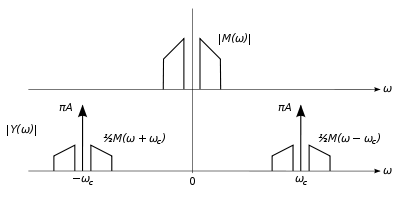
\includegraphics[scale=0.75]{AM_spectrum.png}
\end{center}

For this sake of this picture I found on the internet, the frequency space representations of the original signal and modulated signal are $M(\omega)$ and $Y(\omega)$ respectively. The Fourier transform of the original signal is convolved with the two delta functions that define a pure harmonic at frequency $\omega_c$

\textbf{Demodulation:}\\ 
Mathematically, we can demodulate an AM signal in a very simple and intuitive way, (in practice the circuits that perform this action are not so simple). \\

Suppose we multiply our one band of our modulated signal by a pure harmonic of the same frequency and phase as the carrier wave (after filtering out the other parts):
\begin{equation}
\cos{(\omega_c t)}m_b(t)=\cos{(\omega_c t)}\cos{((\omega_c-\omega_0)t)}
\end{equation}
Using the same trigonometric identity as before:
\begin{equation}
\cos{(\omega_c t)}m_b(t) \propto \cos{(2\omega_c t)}+\cos{(\omega_0 t)}
\end{equation}
As you can see the resultant signal has frequency components at $2\omega_c$ (twice the carrier) and $\omega_0$ (the original signal)! We simply need to filter out the high frequency content using an analog low pass filter.



\subsection{Frequency Modulation}
Frequency modulation is another technique used to transfer information on a carrier signal, except this time we modulate the \textit{frequency} of the carrier signal instead of the amplitude.\\

Before discussing the frequency modulation, we need to define the \textbf{instantaneous frequency} of a harmonic wave. Usually, when we think about the frequency of a wave, we think about the following:
\begin{equation}
y(t)=\cos{(2\pi f t)}
\end{equation}
Where the frequency of this harmonic wave is $f$. Taking the derivative of our signal \textit{pulls out} the frequency:
\begin{equation}
\dot{y}(t)=-2\pi f\sin{(2\pi f t)}
\end{equation}
So what if we have a signal of the following form:
\begin{equation}
y(t)=\cos{\big(2\pi \int_0^{t}d\tau \;  f(\tau)\big)}
\end{equation}
And take the derivative to \textit{pull out} the frequency:
\begin{equation}
\dot{y}=-2\pi f(t) \sin{\big(2\pi \int_0^{t}d\tau \;  f(\tau)\big)}
\end{equation}
By this understanding, the frequency is $f(t)$, and is referred to as the \textbf{instantaneous frequency} of the harmonic.\\

With this method of thinking, we are now ready to understand frequency modulation as changing the instantaneous frequency of a carrier wave! Suppose the carrier wave was intrinsic frequency $f_c$, and we would like to modulate it with a signal $s(t)$.
\begin{equation}
f_c = \text{carrier frequency} \: \: \: \: \: \& \: \: \: \: \: s(t) = \text{information to be transmitted}
\end{equation}
If we want to modulate the frequency of our carrier, we should define the instantaneous frequency as follows:
\begin{equation}
f(t) = f_c + f_\Delta s(t)
\end{equation}
Now putting it all in a harmonic wave we get the following modulated signal:
\begin{equation}
y(t)=\cos{\big(2\pi \int_0^{t}d\tau \;  (f_c+f_\Delta s(\tau))\big)}
\end{equation}
Where the instantaneous frequency changes with $s(t)$! The value constant value $f_\Delta$ is referred to as the \textit{frequency deviation}, and determines the sensitivity of our carrier frequency to our information signal.\\

So what does this look like for a simple sine wave information signal with frequency $f_m$? 
\begin{equation}
s(t) = A_m \cos{(2\pi f_m t)}
\end{equation}
\begin{equation}
\int_{0}^{t}d\tau \; s(\tau) = A_m \frac{\sin{(2\pi f_m t)}}{2\pi f_m}
\end{equation}
After evaluating the modulation equation our final signal will be of the form:
\begin{equation}
y(t)=\cos{\big(2\pi f_c t+\frac{f_\Delta A_m}{f_m} \sin{(2\pi f_m t)}\big)}
\end{equation}

To get a better sense of what this signal would actually look like, see \href{https://www.desmos.com/calculator/oapme28nfh}{here}.

\subsection{Phase Modulation}
Phase modulation is very similar to frequency modulation, except we simply don't integrate our information signal, (therefore modifying the phase of the carrier wave instead of the frequency).\\

Just like in AM and FM, we will have a carrier harmonic with angular frequency $\omega_c$, of which we will modulate the phase our signal $s(t)$:
\begin{equation}
y(t)=\cos{\big(\omega_ct+A_m s(t) \big)}
\end{equation}

If we take our information to be another harmonic of frequency $\omega_i$, the modulated signal looks very familiar to FM:
\begin{equation}
y(t)=\cos{\big(\omega_ct+A_m \cos{(\omega_i t)} \big)}
\end{equation}

A great visual representation of a phase modulated signal can be found \href{https://upload.wikimedia.org/wikipedia/commons/a/ae/Phase-modulation.gif}{here}

\subsubsection{Binary Phase Shift Keying}
One of the more simple means of transferring digital data using phase modulation is known as Binary Phase Shift Keying (BPSK). If the information we wish to transmit is simply a sequence of bits, then the function describing our modulated signal becomes much simpler:
\begin{equation}
y(t)=\cos{\big(\omega_ct + \pi (n-1) \big)} \; \; \; \; \; \text{ where } \; \; \; n \in \{0,1\}
\end{equation}
Where $n$ represents the value of the bit sequence we wish to transfer! A visual depiction of what such a signal would look like is shown below:
\begin{center}
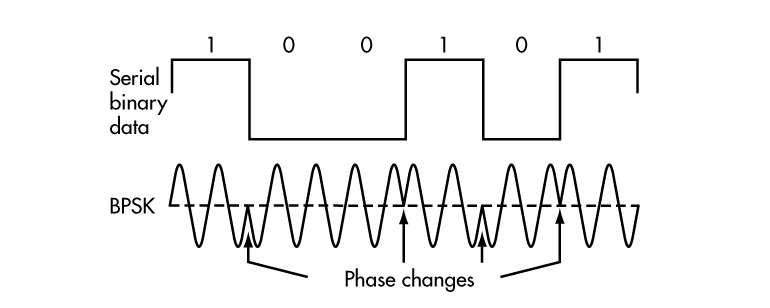
\includegraphics[scale=0.45]{BPSK.png}
\end{center}


\section{Other Applications}
\subsection{Spectrum Smearing \& Windowing}
\subsubsection{Spectrum Smearing}
The Discrete Fourier Transform is an extremely useful tool, although it has limitations. When taking the Discrete Fourier Transform of a signal, the signal must be of a finite length, and the finite length signal is assumed to be periodic by the machinery of the DFT.\\

When taking the DFT of a signal, we are decomposing it into a sum of harmonics of the same period. For example, when taking the DFT of the following signal (assume discrete):
\begin{center}
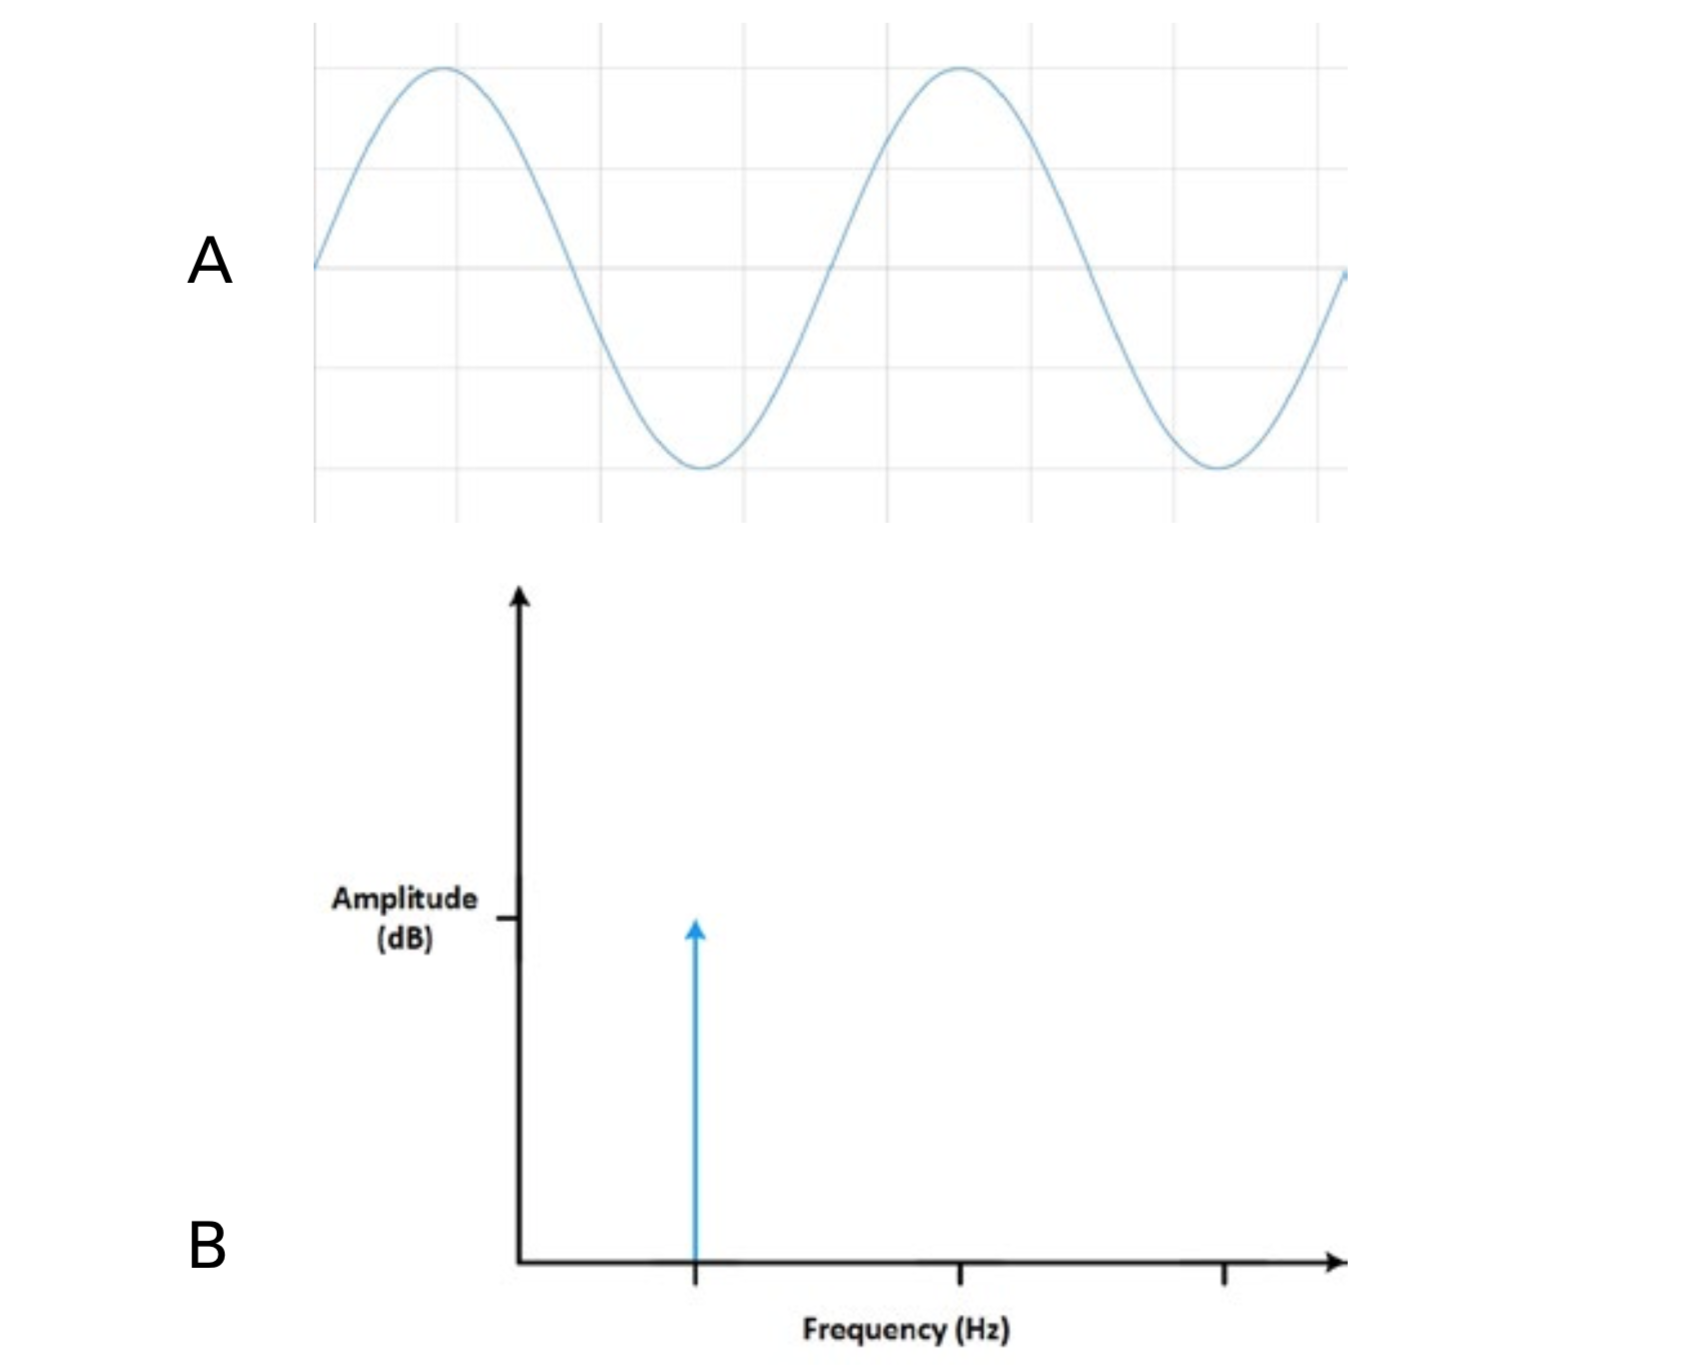
\includegraphics[scale=0.45]{int_periods.png}
\end{center}
There is a single value in the frequency space because signal A (assumed to be periodic), is clearly made up of a sine wave of a certain frequency. Now, what happens if we take the DFT of the following signal (which is also assumed to be periodic):
\begin{center}
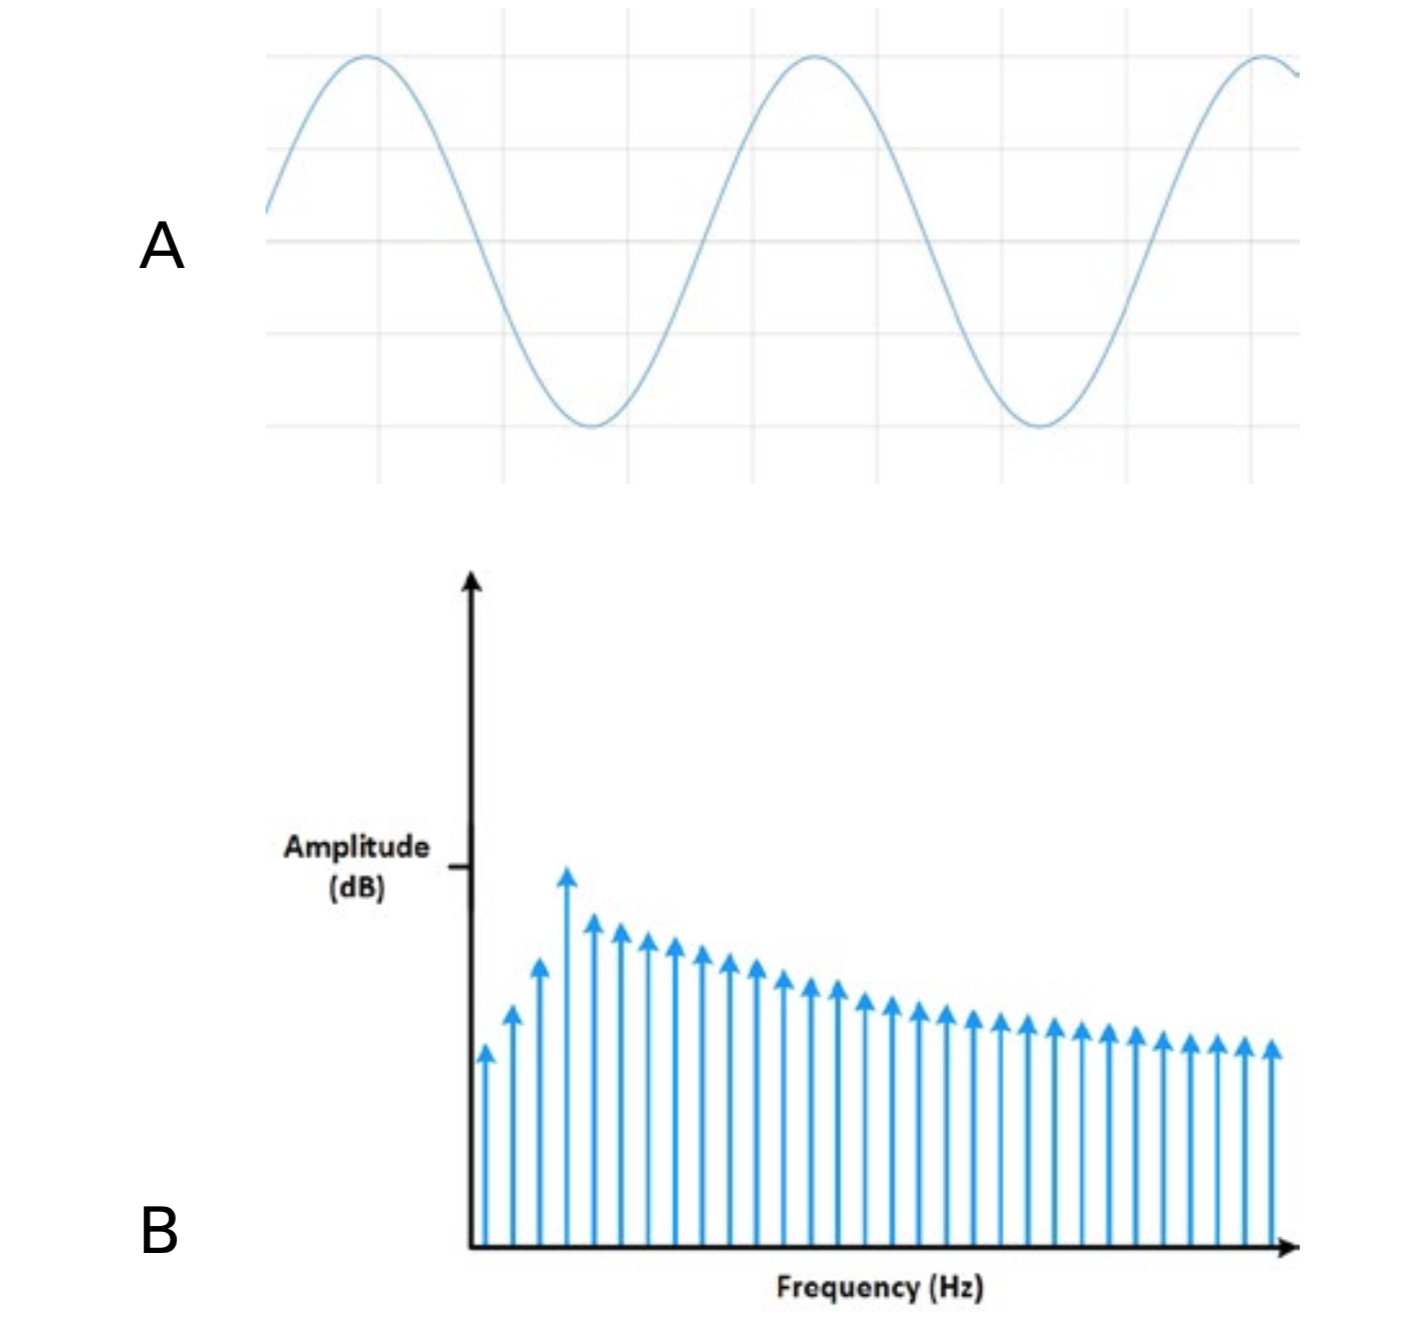
\includegraphics[scale=0.45]{non_int_periods.png}
\end{center}
If the signal (A) is assumed to be periodic, and there is a non-integer number of periods of the signal wave present, the signal the DFT sees will be discontinuous! This new discontinuous signal is decomposed into harmonics that are continuous over the boundary, resulting in what is known as \textbf{spectrum smearing} or \textbf{spectral leakage}. The correct frequency is near the peak (but not properly captured by the DFT). The DFT is obviously not representative of the frequencies actually present in our signal.\\

\subsubsection{Windowing}
One possible method of dealing with the issue of spectral leaking intrinsic to the DFT is known as \textbf{windowing}. Windowing is the multiplying of the finite length signal of interest by a \textit{window function}, which minimizes the effect of discontinuities.\\

One of the more common window functions is known as the Hanning Window, and takes the following form:
\begin{equation}
w[n]=\sin^{2}{(\frac{\pi n}{N-1})}
\end{equation}
\begin{center}
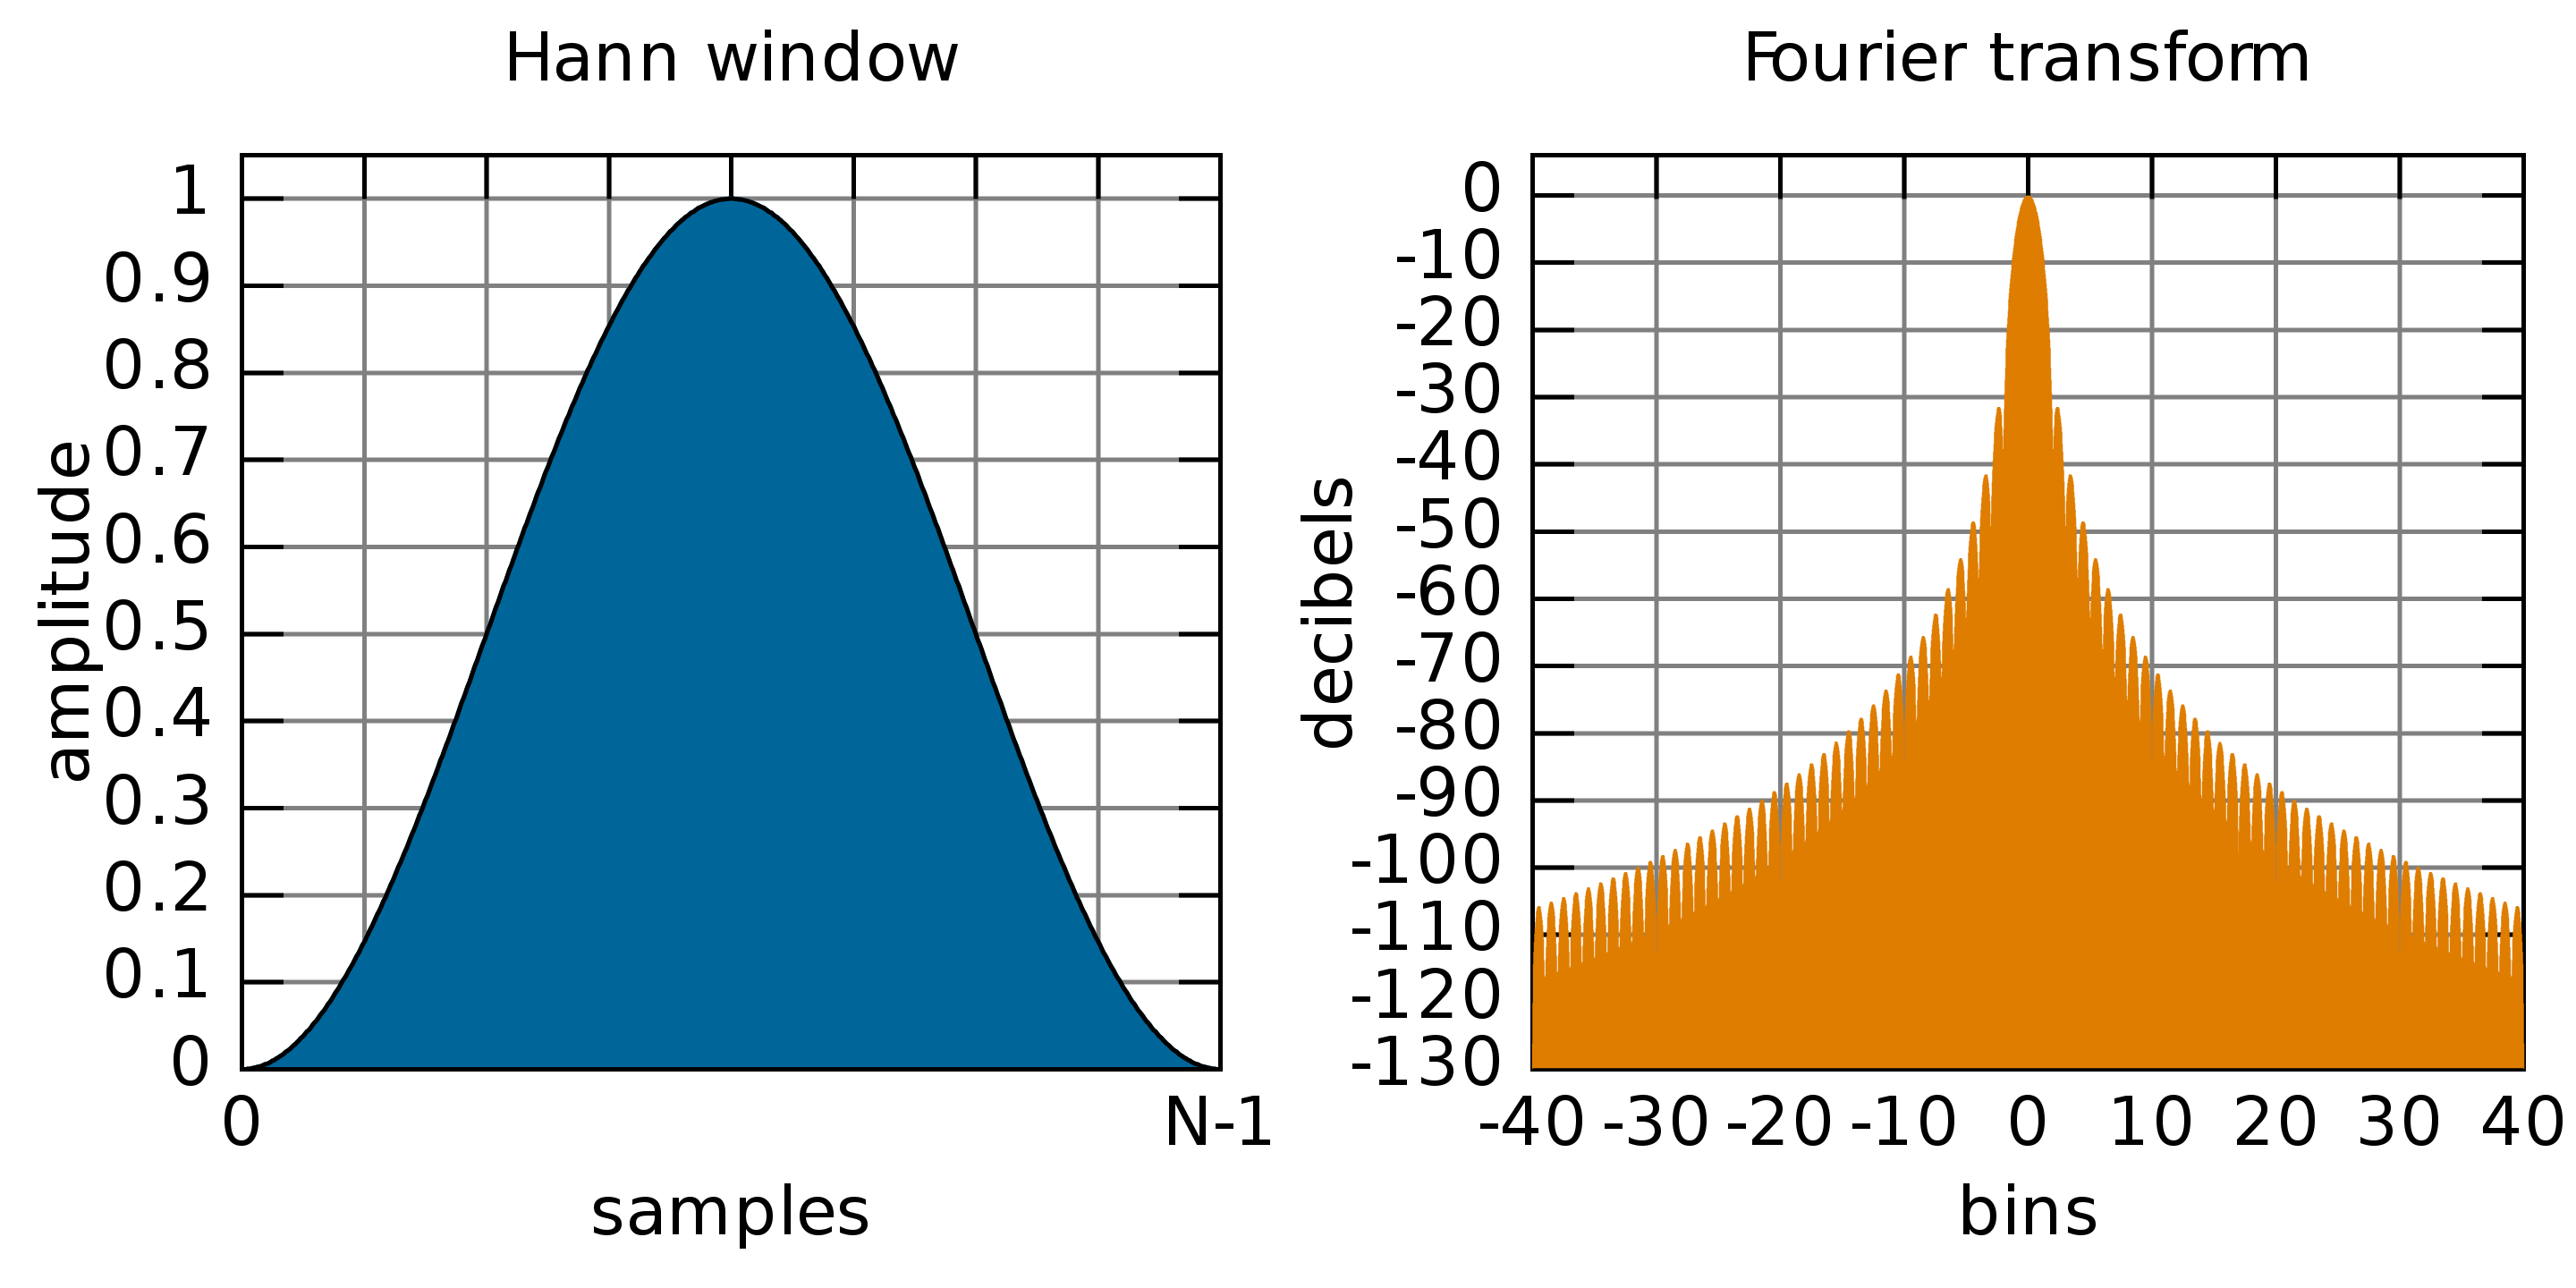
\includegraphics[scale=0.15]{HannWindow.png}
\end{center}
Since this signal is zero valued at 0 and $N-1$, and also has zero valued first derivative at 0 and $N-1$, the affects of discontinuities on the frequency spectrum of the DFT are lessened. The effect of multiplying a signal by a Hanning is easily visualized by the following:
\begin{center}
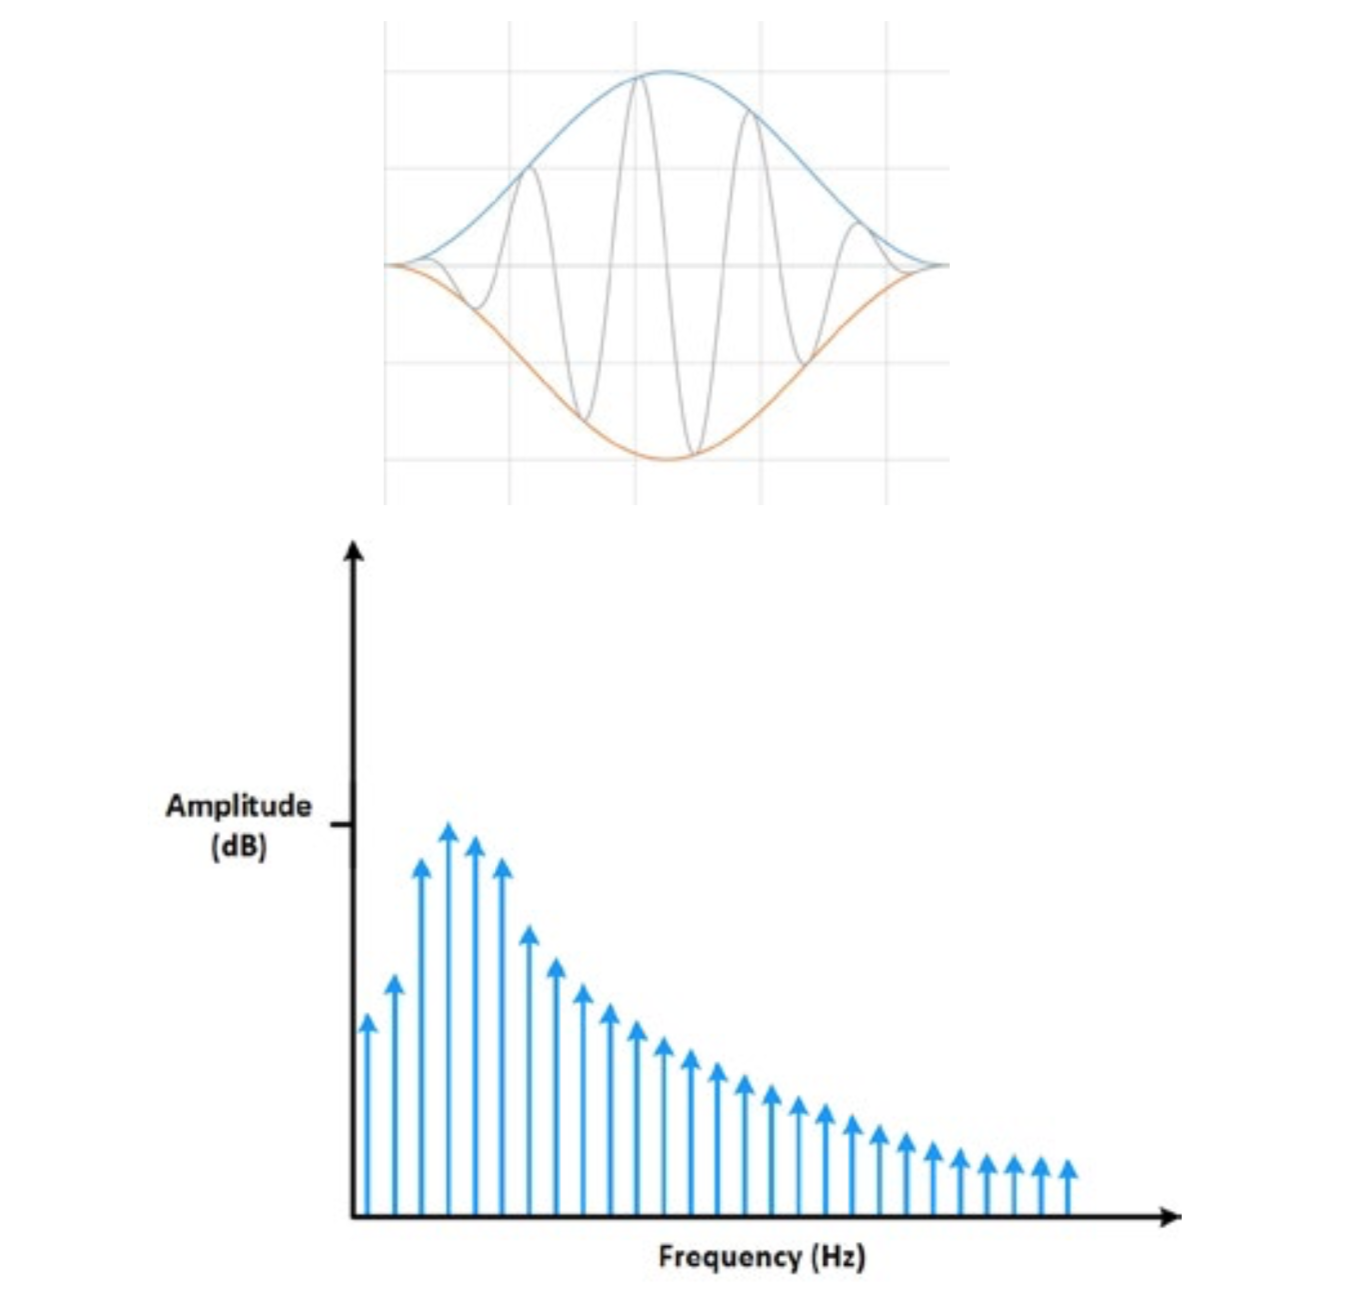
\includegraphics[scale=0.55]{HannEffect.png}
\end{center}
The unwanted frequencies are visibly reduced in power after the discontinuities are minimized. 

\subsection{Fast Fourier Transform}
The method of calculating the DFT of a finite length signal is on the order of $O(n^2)$ when given simply as: 
\begin{equation}
\hat{X}[k']=\sum_{n=0}^{N-1}x[n]e^{-j2\pi k' n/N}
\end{equation}
This is very inefficient, and scales quickly as $n$ increases. We can improve the efficient by taking advantage of symmetries within the DFT. \textbf{Remember that the DFT is periodic in $k$}, $X[k]=X[k+N]$. \\

Suppose we assume our signal length is a power of 2, $N=2^m$, and split up the DFT calculation into even and odd valued $n$ as follows:
\begin{equation}
\hat{X}[k]=\underbrace{\sum_{n=0}^{N/2-1}x[2n]e^{-j2\pi k 2n/N}}_{\text{even }n}+\underbrace{\sum_{n=0}^{N/2-1}x[2n+1]e^{-j2\pi k (2n+1)/N}}_{\text{odd } n}
\end{equation}
\begin{equation}
\hat{X}[k]=\underbrace{\sum_{n=0}^{N/2-1}x[2n]e^{-j2\pi k n/(N/2)}}_{\text{even }n}+\underbrace{e^{-j2\pi k/N}\sum_{n=0}^{N/2-1}x[2n+1]e^{-j2\pi k /(N/2)}}_{\text{odd } n}
\end{equation}
We are in fact taking the length $N/2$ DFT of the even and odd parts of our original length $N$ signal, and multiplying the odd part by a phase factor. Rewriting in simpler terms after denoting the even and odd valued DFTs as $E$ and $O$ respectively:
\begin{equation}
\hat{X}[k] = E[k] + e^{-j2\pi k/N}O[k]
\end{equation}
Remember, since $E[k]=E[k+N/2]$ and $O[k]=O[k+N/2]$, only the phase factor has different values for $k<N/2$ and $k>N/2$. When applied recursively to calculate $E[k]$ and $O[k]$, we have significantly reduced the asymptotic runtime of the DFT to $O(n \log(n))$. You will write your own FFT algorithm and compare the speed to your original DFT as homework.

\subsection{Time-Frequency Uncertainty Principle}
One extremely important aspect of frequency analysis is known as the \textbf{time-frequency uncertainty principle}, (although many different variables have a finite uncertainty).\\

The most familiar uncertainty principle from quantum mechanics between a particle's position $x$ and momentum $p$, formally stated as:
\begin{equation}
\sigma_x \sigma_p \geq \frac{\hbar}{2}
\end{equation} 
Where $\sigma_x$ and $\sigma_p$ are the standard deviations of the position and momentum of a particle respectively, and $\hbar$ is the reduced Planck constant. We will obviously not go into the derivation of this lower bound (take 8.04/8.05 to do that!).\\

We can take this familiar uncertainty principle and manipulate it until we have an uncertainty between time and frequency. In quantum mechanics, momentum is equal to $\hbar$ multiplied by angular spatial frequency:
\begin{equation}
p=\hbar \omega_{s}
\end{equation}
Since the standard deviation scales in magnitude with the distribution of interest (taking $X$ to be some distribution):
\begin{equation}
\sigma[X]=\sigma_x \Longleftrightarrow \sigma[aX]=|a|\sigma_x
\end{equation}

The quantum uncertainty relation between position and momentum can be rewritten as follows:
\begin{equation}
\sigma_x \hbar  \sigma_{\omega_s} \geq \frac{\hbar}{2}
\end{equation} 
\begin{equation}
\sigma_x \sigma_{\omega_s} \geq \frac{1}{2}
\end{equation} 
We can \textit{informally} convert the distributions of space $x$ and spatial angular frequency $\omega_x$ to distributions of time, leaving us with the time-frequency uncertainty principle:
\begin{equation}
\boxed{
\sigma_t \sigma_{\omega} \geq \frac{1}{2}}
\end{equation} 
Stated as follows: \textbf{the standard deviation of a signal as a function of time multiplied by the standard deviation of the same signal as a function of angular frequency is greater than or equal to $1/2$}.\\

This may seem very abstract, but \href{https://www.desmos.com/calculator/ebjkfeufmd}{this} interactive visualization of a Guassian signal may help your understanding.

\end{document}